\documentclass[twoside]{article}
% \documentclass[a4paper,10pt,twoside]{article}
\usepackage{afterpage}			% met landscape sans blanc
\usepackage[british]{babel}
\usepackage{caption}
\usepackage{color}			% Gestion de la couleur
\usepackage{fancyhdr}			% en-tête et pied-de-page
\usepackage{graphicx} 			% Insère image (eps, ps)
\usepackage{hyperref}			% Gère les liens hypertexte
\usepackage[utf8]{inputenc}
\usepackage{longtable}
\usepackage{lscape}			% Format landscape
\usepackage[round]{natbib}		% Bibliographie
\usepackage{pxfonts}
\usepackage[load-configurations = abbreviations]{siunitx}
\usepackage[skip=10pt]{subcaption}	% Figure composite
\usepackage{textcomp}
\usepackage{url}

\usepackage{geometry}
 \geometry{
 a4paper,
 total={210mm,297mm},
 left=20mm,
 right=20mm,
 top=20mm,
 bottom=20mm,
 }
 
 \newcommand\registred{\textsuperscript{\tiny\textregistered}}
 

%%%%%%%%%%%%%%%%%%%%%%%%%%%%%%%%%%%%%%%%%%%%%%%%%%%%%%%%%%%%%%%%%%%%
%% Folders
%%%%%%%%%%%%%%%%%%%%%%%%%%%%%%%%%%%%%%%%%%%%%%%%%%%%%%%%%%%%%%%%%%%%

\graphicspath{
	{/home/jeremy/UniGE/Publication/Ragusa2017a/figs/}
	{/home/jeremy/UniGE/Publication/Ragusa2017a/graphs/}
	}

%%%%%%%%%%%%%%%%%%%%%%%%%%%%%%%%%%%%%%%%%%%%%%%%%%%%%%%%%%%%%%%%%%%%
%% Links
%%%%%%%%%%%%%%%%%%%%%%%%%%%%%%%%%%%%%%%%%%%%%%%%%%%%%%%%%%%%%%%%%%%%

\definecolor{vert}{RGB}{32,121,35}
\definecolor{mauve}{RGB}{120,29,94}
\definecolor{navy}{RGB}{0,95,190}
\urlstyle{sf} \hypersetup{
	unicode = true,
	colorlinks = true,
	urlcolor = mauve,
	linkcolor = {navy},
	citecolor = vert,
	pdfauthor = {Jérémy Ragusa, Pascal Kindler, Branimir Segvic, Lina Maria Ospina‐Ostios},
	pdftitle = {Provenance analysis of the Voirons Flysch (Gurnigel nappe, Haute-Savoie, France): stratigraphic and palaeogeographic implications},
	pdfsubject = {},
	pdfkeywords = {Gurnigel nappe, Chablais Prealps, Voirons Flysch, Provenance, QEMSCAN, Heavy-mineral, Valais domain},
	pdfcreator = {Jérémy Ragusa},
	pdfproducer = {LaTeX et pdflatex}
	}
	
%%%%%%%%%%%%%%%%%%%%%%%%%%%%%%%%%%%%%%%%%%%%%%%%%%%%%%%%%%%%%%%%%%%%
%% Headers and Footers
%%%%%%%%%%%%%%%%%%%%%%%%%%%%%%%%%%%%%%%%%%%%%%%%%%%%%%%%%%%%%%%%%%%%

\fancypagestyle{plain}{
	\fancyhead[LO]{Int J Earth Sci (Geol Rundsch)}
	\fancyhead[RO]{DOI:10.1007/s00531-017-1474-9}
	\renewcommand{\headrulewidth}{0.4pt}
	}
	
\fancyhead[LO]{Int J Earth Sci (Geol Rundsch) (2017) 106:2619--2651}
\fancyhead[RO]{\thepage}
\fancyhead[RE]{Int J Earth Sci (Geol Rundsch) (2017) 106:2619--2651}
\fancyhead[LE]{\thepage}
\fancyfoot{}
\pagestyle{fancy}

%%%%%%%%%%%%%%%%%%%%%%%%%%%%%%%%%%%%%%%%%%%%%%%%%%%%%%%%%%%%%%%%%%%%
%% Units
%%%%%%%%%%%%%%%%%%%%%%%%%%%%%%%%%%%%%%%%%%%%%%%%%%%%%%%%%%%%%%%%%%%%

\sisetup{detect-all,
	 inter-unit-separator=$\cdot$,
	 range-phrase=--, % Utilise le tiret court pour dire "de... à"
	 range-units=single, % Cache l'unité sur la première borne
	}

\DeclareSIUnit{\tour}{tr}
\DeclareSIUnit{\tourperminute}{\tour\per\minute}
\DeclareSIUnit{\Ma}{Ma}

%%%%%%%%%%%%%%%%%%%%%%%%%%%%%%%%%%%%%%%%%%%%%%%%%%%%%%%%%%%%%%%%%%%%
%% Bibliography
%%%%%%%%%%%%%%%%%%%%%%%%%%%%%%%%%%%%%%%%%%%%%%%%%%%%%%%%%%%%%%%%%%%%

\setlength{\bibsep}{0.1cm}		% Intervalle entre références
\bibpunct{(}{)}{ ;}{a}{,}{,} 		% Mise en forme références

%%%%%%%%%%%%%%%%%%%%%%%%%%%%%%%%%%%%%%%%%%%%%%%%%%%%%%%%%%%%%%%%%%%%

\title{Provenance analysis of the Voirons Flysch (Gurnigel nappe, Haute-Savoie, France): stratigraphic and palaeogeographic implications}
\author{Jérémy Ragusa\textsuperscript{1}, Pascal Kindler\textsuperscript{1}, Branimir Segvic\textsuperscript{2}, Lina Maria Ospina‐Ostios\textsuperscript{3}}
\date{}
\begin{document}

\maketitle

{\smallskip{\footnotesize%
  \textsuperscript{1} \textsc{University of Geneva, Department of Earth Sciences, 13, Rue des Maraîchers, CH-1205 Geneva, Switzerland}\par  
  \textit{Contact}: J\'er\'emy~Ragusa (\texttt{\url{jeremy.ragusa@unige.ch}})\par
  \addvspace{\medskipamount}
  \textsuperscript{2} \textsc{Texas Tech University, Department of Geosciences, 1200 Memorial Circle, Lubbock, TX 79409, USA}\par
  \addvspace{\medskipamount}
  \textsuperscript{3} \textsc{Universidad del Valle, Escuela de Ingeniería Civil y Geomática, Cali, Colombia}\par
}}

\begin{abstract}
The Chablais Prealps (Haute-Savoie, France) represent a well-preserved accretionary wedge of the Western Alpine Tethys. They comprise a stack of sedimentary nappes related to palaeogeographic realms ranging from the Ultrahelvetic to the Southern Penninic. The provenance analysis is based on the Gazzi-Dickinson method, and on QEMSCAN\registred\ for heavy-minerals. The Quartzose petrofacies is the most important of the two sources, and supplied three of the four formations of the Voirons Flysch. It is similar to the sources that fed the other flyschs from the Gurnigel nappe. It is characterised by a mature, quartz-rich assemblage and a heavy mineral population dominated by apatite and the zircon-tourmaline-rutile mineral group. These observations suggest a Clastic wedge provenance. The Feldspathic petrofacies is derived from a feldspar-rich source associated with metamorphic clasts and a heavy mineral population dominated by garnet. This provenance characterises only one formation of the Voirons Flysch, and is related to the Axial Belt provenance.\par
This provenance analysis shows that the Middle Eocene to Early Oligocene Voirons Flysch was fed by two sources, in contrast to the other flyschs of the Gurnigel nappe, and further suggests that this flysch was not deposited in the Piemont Ocean but in the Valais domain. Based on the results and comparative provenance analysis with the other flyschs of the Gurnigel nappe, we propose a generic feeding model which involves the Sesia-Dent Blanche nappe, the sedimentary nappes incorporated in the accretionary prism, and probably the Briançonnais basement.
\end{abstract}

{\bf Keywords:} Gurnigel nappe, Chablais Prealps, Voirons Flysch, Provenance, QEMSCAN\registred, Heavy-mineral, Valais domain

\section{Introduction}

The Alps are one of the most studied mountain chains in the world, and recent palaeogeographic reconstitutions have shed light on the distribution of tectonic units and the timing of their incorporation into the orogenic belt \citep{Schmid1996,Schmid2004,Stampfli2002a,Stampfli2002b,Handy2010}. The palaeogeographic reconstructions of sedimentary covers are partly based on age data, with the youngest age indicating the end of sedimentation in the basin and its subsequent incorporation into the accretionary prism \citep{Stampfli2002b}. Most of these youngest and highest sedimentary successions essentially consist of flysch deposits. Provenance studies on the extrabasinal detrital fraction of these flyschs are highly used for palaeogeographic reconstructions. These studies normally rely on petrographic and mineralogical analogies with hypothesised source materials \citep{Eynatten1999,Beltran-Trivino2013} which help to establish the sedimentary flux and to estimate the successive exhumation of the detrital sources through time \citep{Trautwein2001a}. The techniques of provenance analysis have markedly improved in the last decades with the refinement of the tectonic settings of the source rocks \citep{Dickinson1979a,Dickinson1983,Dickinson1985}, the development of statistical tools to constrain the sediment source \citep{Garzanti2004,Garzanti2007a,Garzanti2007b,Garzanti2010} and the geochemistry of single grains \citep{Eynatten2012}.\par
\medskip

\afterpage{
	\begin{figure}[htp!]
		\centering
		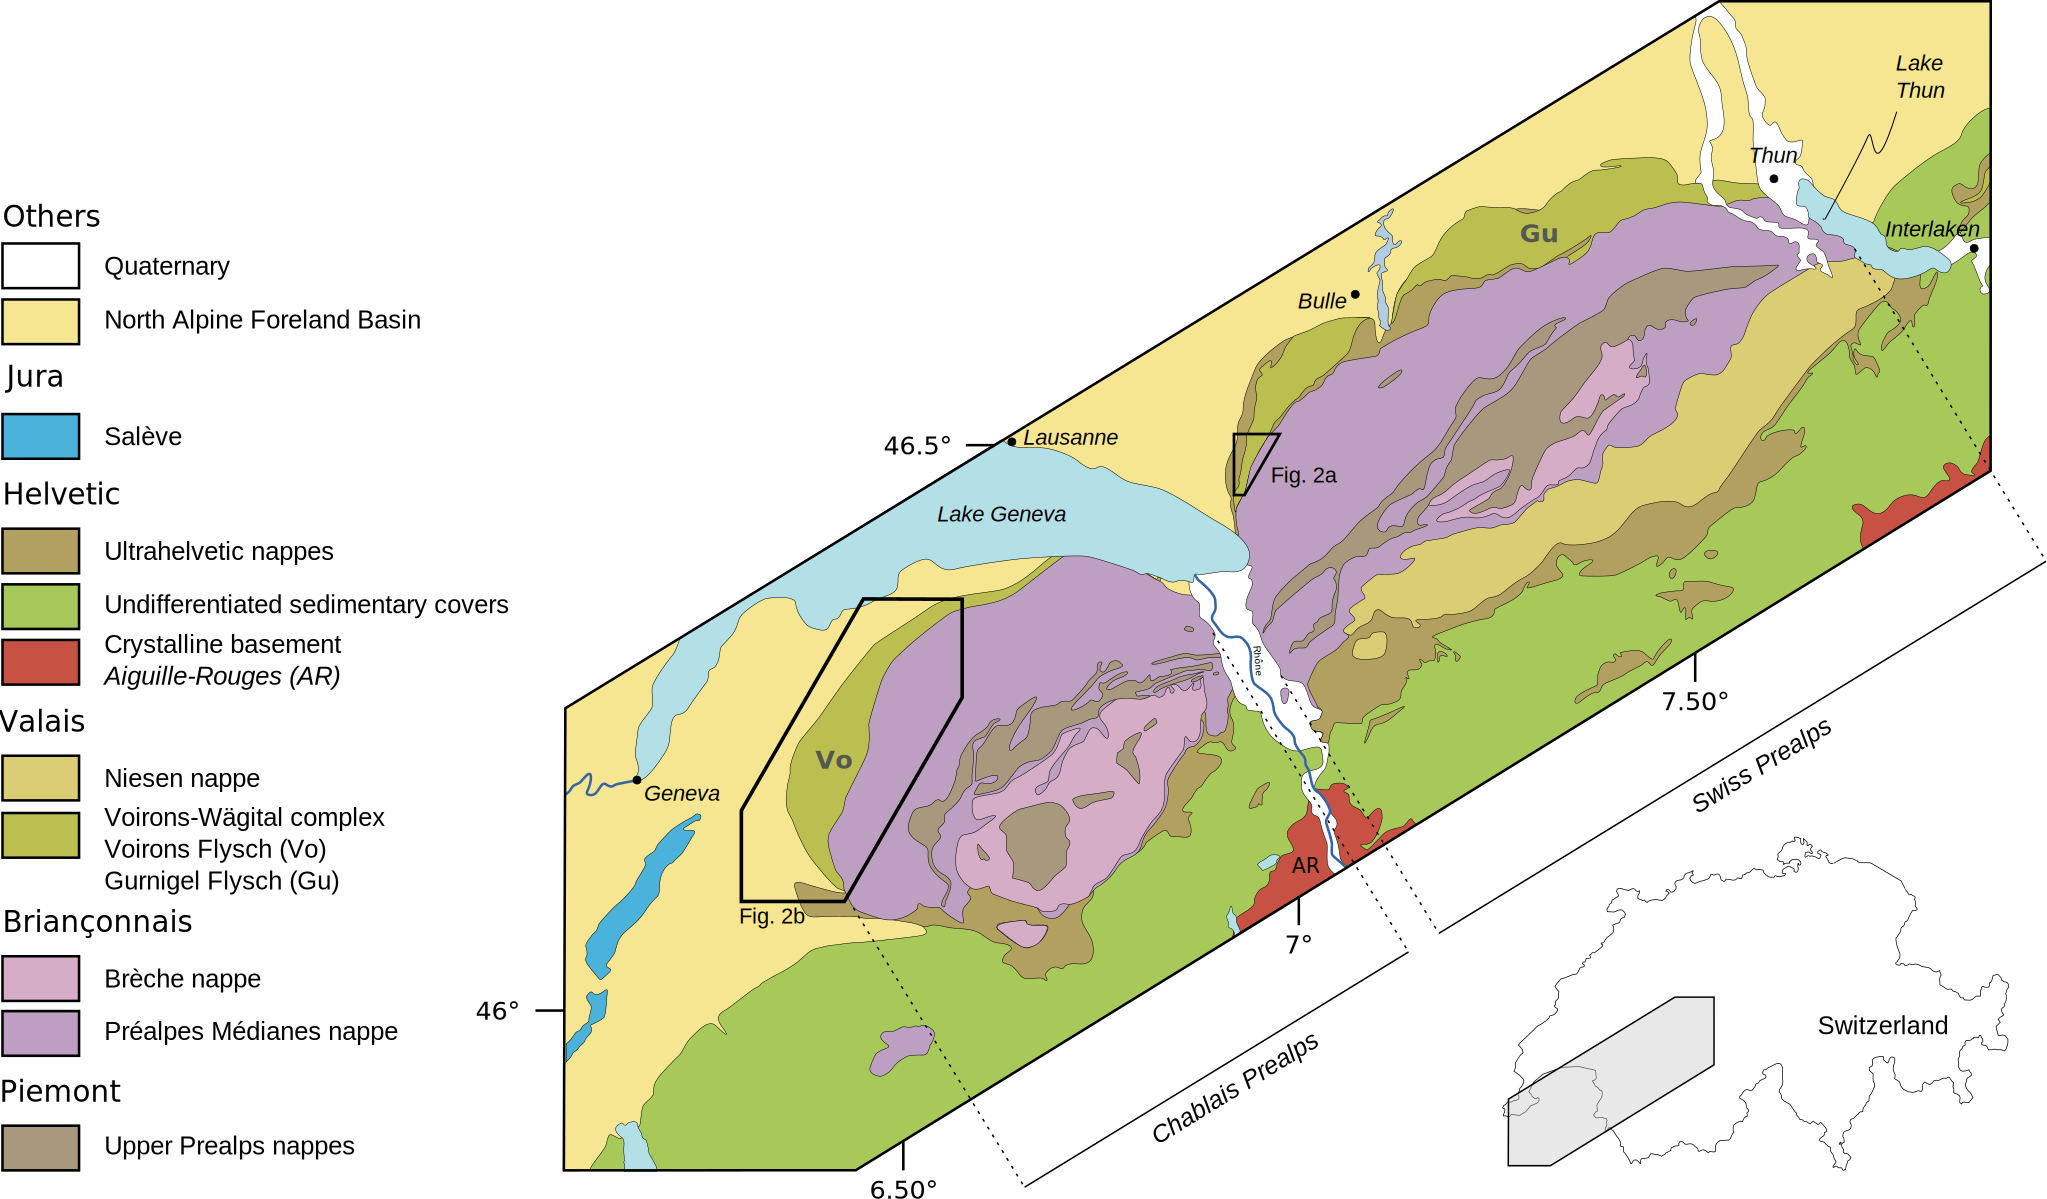
\includegraphics[width=\textwidth]{Fig1.pdf}
		\caption{Tectonic map of the Chablais and Swiss Prealps \citep[modified]{SwissTopo2008} with the location of the different flyschs of the Gurnigel nappe. The black box indicates the studied area described in Fig.~\ref{fig:Fig4}.}
		\label{fig:Fig1}
	\end{figure}
	}

In the Alps, many sedimentary cover nappes are separated from their crystalline basement which complicates the identification of their original palaeogeographic location. In particular, the palaeo-depositional realm of the Cretaceous to Eocene Gurnigel nappe, a flysch nappe now exposed in the Swiss and French Prealps (Fig.~\ref{fig:Fig1}), is most controversial, as it has been successively placed in the Ultrahelvetic domain \citep{Lombard1940a,Hsu1960,Trumpy1960,Hubert1967,Hsu1971}, along the southern margin of the Piemont Ocean \citep{Caron1976,Winkler1983,Winkler1984}, and, more recently, in the Valais trough \citep{Trumpy2006,Ospina-Ostios2013,Ragusa2015} (Fig.~\ref{fig:Fig2}).\par
\medskip
The goal of this study is to analyse the framework composition and heavy-mineral assemblage of the Middle Eocene to Early Oligocene Voirons Flysch which corresponds to the western extension of the Gurnigel nappe in France (Fig.~\ref{fig:Fig1}). These new data provide unsuspected information on the source regions of this flysch, and help in refining its stratigraphical context. Data are further compared with similar results from other parts of the Gurnigel nappe and from various Prealps flyschs (Figs.~\ref{fig:Fig1} and~\ref{fig:Fig2}; \citealp{Caron1989}), and finally are used to formulate an original palaeogeographic model for the Voirons Flysch.\par

\afterpage{
	\begin{figure}[htp!]
		\centering
		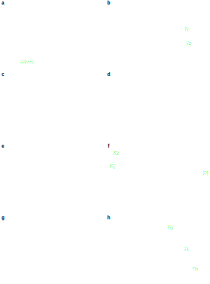
\includegraphics[width=\textwidth]{Fig2.pdf}
		\caption{Simplified palinspastic model from Stampfli et al. (1998, modified) with the original location of the Prealps nappes. Stars represent the successive paleogeographic attribution of the Gurnige nappe: Ultrahelvetic realm (white), South Penninic (black) and Valais domain (purple).}
		\label{fig:Fig2}
	\end{figure}
	}

\section{Geological background}

The Prealps form moderately elevated reliefs (ca. 2 000 m) between Lake Geneva and Lake Zurich (Fig.~\ref{fig:Fig1}). They include, in particular, the Chablais massif, south of Lake Geneva, and the Swiss Prealps, between Lake Geneva and Lake Thun. These reliefs encompass a stack of sedimentary cover nappes detached from their respective basement during the Alpine subduction, and follow a thin-skinned, in-sequence thrusting (Figs.~\ref{fig:Fig1} and~\ref{fig:Fig3}; \citealp{Mosar1991,Wissing2002}. They represent the former sedimentary accretionary to orogenic prism of the Alpine Tethys in this part of the Western Alps \citep{Stampfli1998,Handy2010}. Nowadays, they overlie the Helvetic nappes to the SE and the North Alpine Foreland Basin (NAFB) to the NW (Fig.~\ref{fig:Fig1}). Due to the NW translation of both of these units, the frontal edge of the Prealps includes tectonic slices from the Helvetic nappes (e.g. the Subalpine Flysch) and from the subsequent filling-up of the NAFB (e.g. the Subalpine Molasse). These units are separated from the Prealps nappes by the Infraprealpine mélange (Fig.~\ref{fig:Fig4}; \citealp{Jeanbourquin1992}.\par
\medskip

\afterpage{
	\begin{figure}[htp!]
		\centering
		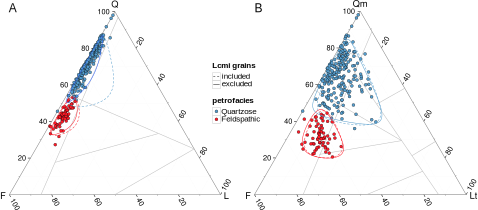
\includegraphics[width=\textwidth]{Fig3.pdf}
		\caption{Cross-section of the Chablais Prealps from Caron (1972, modified).}
		\label{fig:Fig3}
	\end{figure}
	}

The Gurnigel nappe is one of the lowermost nappes of the Prealps, and is exposed along their NW edge (Figs.~\ref{fig:Fig1} and~\ref{fig:Fig3}). It comprises several flysch units generally interpreted as gravity-flow deposits: Voirons \citep{Lombard1940a,Ospina-Ostios2013,Ragusa2015}, Fayaux \citep{Stuijvenberg1976,Weidmann1976a,JanduChene1977,Weidmann1985}, Niremont \citep{Morel1980,Ambrosetti2005}, Berra \citep{Tercier1928a}, Gurnigel \citep{Stuijvenberg1979}, Schlieren \citep{Winkler1983,Winkler1984,Winkler1993} and Wägital \citep{Winkler1985b}. These different flysch successions share similar lithostratigraphic characteristics. Indeed, previous mineralogical studies in the Gurnigel \citep{Stuijvenberg1979}, Schlieren \citep{Winkler1983,Winkler1984} and Wägital \citep{Winkler1985b} flyschs show that constituent rocks are characterised by a quartz-feldspar dominated modal composition with subordinate lithics and a heavy-mineral population dominated by zircon-tourmaline-rutile (ZTR) and garnet \citep{Wildi1985}. The presence of peculiar agglutinated foraminifers (Rhabdamina fauna; \citealp{Brouwner1965,Weidmann1967a,Stuijvenberg1976,Ujetz1996}), the nature of bioturbations \citep{Crimes1981}, and the sedimentological features \citep{Kuenen1953}, all suggest a deep-marine sedimentary environment for these successions. Early biostratigraphic studies based on calcareous nannofossils, dinoflagellates and, more rarely, on planktonic foraminifers indicated a Late Maastrichtian to Lutetian age for all flysch units of the Gurnigel nappe \citep{Rigassi1958,Kuhn1972,JanduChene1975c,JanduChene1977,Stuijvenberg1979,Winkler1983,Winkler1984,Winkler1990,Kaenel1989}. Such an age range is also supported by the occurrence of bentonite layers dated from the Paleocene in the lower part of the Schlieren Flysch \citep{Winkler1985a,Koch2015}, and possibly related to the North Atlantic events \citep{Egger2005}. However, planktonic foraminifers of Middle to Late Eocene/Early Oligocene age have recently been retrieved from the Voirons Flysch \citep{Ujetz1996,Ospina-Ostios2013}.\par
\medskip
For long, the flysch units outcropping along the NW edge of the Prealps were thought to originate from the Ultrahelvetic realm (e.g. \citealp{Tercier1928a,Lombard1940a}; Fig.~\ref{fig:Fig2}), but several authors had already noticed the petrographical resemblance of some conglomerate clasts found in these units (e.g. pink granite fragments) with several rock bodies exposed in the Southern Alps \citep{Sarasin1894b,Pilloud1936,Lombard1940a,Cogulu1961} such as the Bernina nappe, Canavese zone, Err-Albula granite, Falknis nappe, etc. Later, based on petrographic and biostratigraphic data, \cite{Caron1976} regrouped all these flyschs in a new tectonic unit, the Gurnigel nappe, which he correlated with the Sarine nappe (Upper Prealps nappe, Fig.~\ref{fig:Fig2}) of South-Penninic origin. Detrital grains were thought to originate from the Austroalpine domain \citep{Winkler1983,Caron1989}. The peculiar structural position of the Gurnigel nappe at the base of the Prealps nappe stack was then explained by the overthrusting of the Upper Prealps beyond the front of the Préalpes Médianes nappe, followed by out-of-sequence thrusting of the latter \citep{Mosar1991,Wissing2002}. However, recent structural data from the Iberg Klippe \citep{Trumpy2006} and the younger age found by \cite{Ujetz1996} and \cite{Ospina-Ostios2013} now suggest that the Gurnigel flyschs could have been deposited in the Valais Ocean (Fig.~\ref{fig:Fig2}), which would considerably simplify the kinematics of the Prealps.\par

\section{Study area}

The Voirons Massif, which comprises the western portion of the Gurnigel nappe, is located in the Chablais Prealps, at about 20 km from Geneva (Figs. 1 and 3). It includes a series of smoothed hilltops, which are, in decreasing order of altitude, the Voirons (1480 m), the Grande Combe (1293 m), the Mont Vouan (978 m) and the Allinges Hills (754 m). The latter broadly constitute the eastern limit of the massif. The Voirons Massif is essentially made of flysch deposits \citep{Lombard1940a,JanduChene1975c,Stuijvenberg1980a}, whose stratigraphy has recently been revised (\citealp{Ragusa2015}; Fig. 4). Accordingly, it now comprises four lithostratigraphic units:

\afterpage{
	\begin{figure}[htp!]
		\centering
		\includegraphics[width=0.8\textwidth]{Fig4.pdf}
		\caption{Tectonic map of the Voirons Flysch and associated cross section. The Bruant Sandstone Fm. is not represented in this section. The northern part of the Voirons Flysch is mostly covered by Quaternary deposits and does not outcrop. Beyond the Allinges Hills, outcrops of the Voirons Flysch are rare and the eastern limit is not well constrained.}
		\label{fig:Fig4}
	\end{figure}
	}

\begin{enumerate}
 \item The Voirons Sandstone Formation forms the crest and the eastern flank of the Voirons ridge (Fig. 4). It is a thick (200 to 300 m), sandstone-rich succession with variable amounts of intercalated marls (Figs. 5a and 5b). The base of the unit is marked by a marly succession with calcarenite beds (Fig. 5a) similar to the Hellstät Formation of the Gurnigel Flysch \citep{Tercier1928a,Caron1980,Caron1989}. Some m-thick conglomeratic layers are exposed along the Voirons crest. Described as “local deposits” by \cite{Lombard1940a}, they include the pink granite lithoclasts (Fig. 6a) typical of the flyschs from the Gurnigel nappe \citep{Caron1976}. The Voirons Sandstone Fm. presents a large range of sedimentary deposits from channel to lobe settings \citep{Ragusa2015}. Deposition is constrained between the Middle Eocene and the Early Oligocene (planktonic foraminiferal zones P12 to P19, \citealp{Ospina-Ostios2013}. The contact with the overlying Vouan Conglomerate Fm. is transitional \citep{Ragusa2015}.
 \item The Vouan Conglomerate Formation is exposed along the eastern flank of the Voirons ridge, and forms the neighbouring Mont Vouan (Fig. 4). It is a homogeneous stack (300 - 400 m thick) of coarse pebbly sandstones to matrix-supported conglomerates that are frequently amalgamated (Fig. 5c). They are mostly devoid of marly intervals, and include black sandstone and conglomerate lithoclasts of Paleozoic age (Fig. 6b). Pebbles and cobbles are also randomly distributed in sandy layers. Lateral variation and large scours \citep{Frebourg2006} characterise the Vouan Conglomerate Fm. which is restrained to channel depositional settings \citep{Ragusa2015}. The scarce biostratigraphic data from this unit \citep{Frebourg2006,Ospina-Ostios2013} suggest a Late Eocene – Early Oligocene age (planktonic foraminiferal zones P15 to P20). The contact with the Boëge Marl Fm. is sharp and does not present any tectonic deformation \citep{Ragusa2015}.
 \item The Boëge Marl Formation (synonymous: Saxel Marl Fm.) was defined by \cite{Stuijvenberg1980b}, and comprises the Ludran Hills and the Grande Combe. It is one thick ($>1000 m$), predominantly marly succession, interspersed by cm-thick, sandstone-rich layers. The base is characterised by some dm-thick conglomeratic layers. The sandstone beds show frequent ripples and upper-plane bedding (Fig. 5d). The formation is affected by several tectonic folds and thrusts \citep{Coppo1999,Ragusa2015}. This unit is interpreted as lobe or continental-slope deposits \citep{Winkler1984}. The Boëge Marl Fm. shows a tectonic contact with the Préalpes Médianes nappe in the southern part of the studied area and a stratigraphic (?) contact with the overlying Bruant Sandstone Fm. in the Grande Combe area. Indeed, the progressive upward thickening of sandstone beds suggests a transitional contact. The Boëge Marl Fm. is of late Middle Eocene to Early Oligocene age (\citealp{Ospina-Ostios2013}; planktonic foraminiferal zones P13 to P20).
 \item The Bruant Sandstone Formation \citep{Ragusa2015} consists of dm-thick, sandy beds interspersed by cm-thick, marly intervals. No conglomeratic intervals have been found in this formation, but its upper reaches comprise some microconglomerate layers. Its upper limit corresponds to the tectonic contact with the Préalpes Médianes nappe. From a petrographic viewpoint, the Bruant Sandstone Fm. is comparable to the Voirons Sandstone Fm., and is interpreted as channel to lobe deposits \citep{Ragusa2015}. No biostratigraphic data have so far been retrieved from this unit. The formation thickness is estimated at about 1000 m. Up to now, this unit was incorrectly interpreted as a sedimentary mélange \citep{Kerrien1998} because of the pronounced (tectonic) deformation near the contact with the Préalpes Médianes nappe.
\end{enumerate}

\afterpage{
	\begin{figure}[htp!]
		\centering
		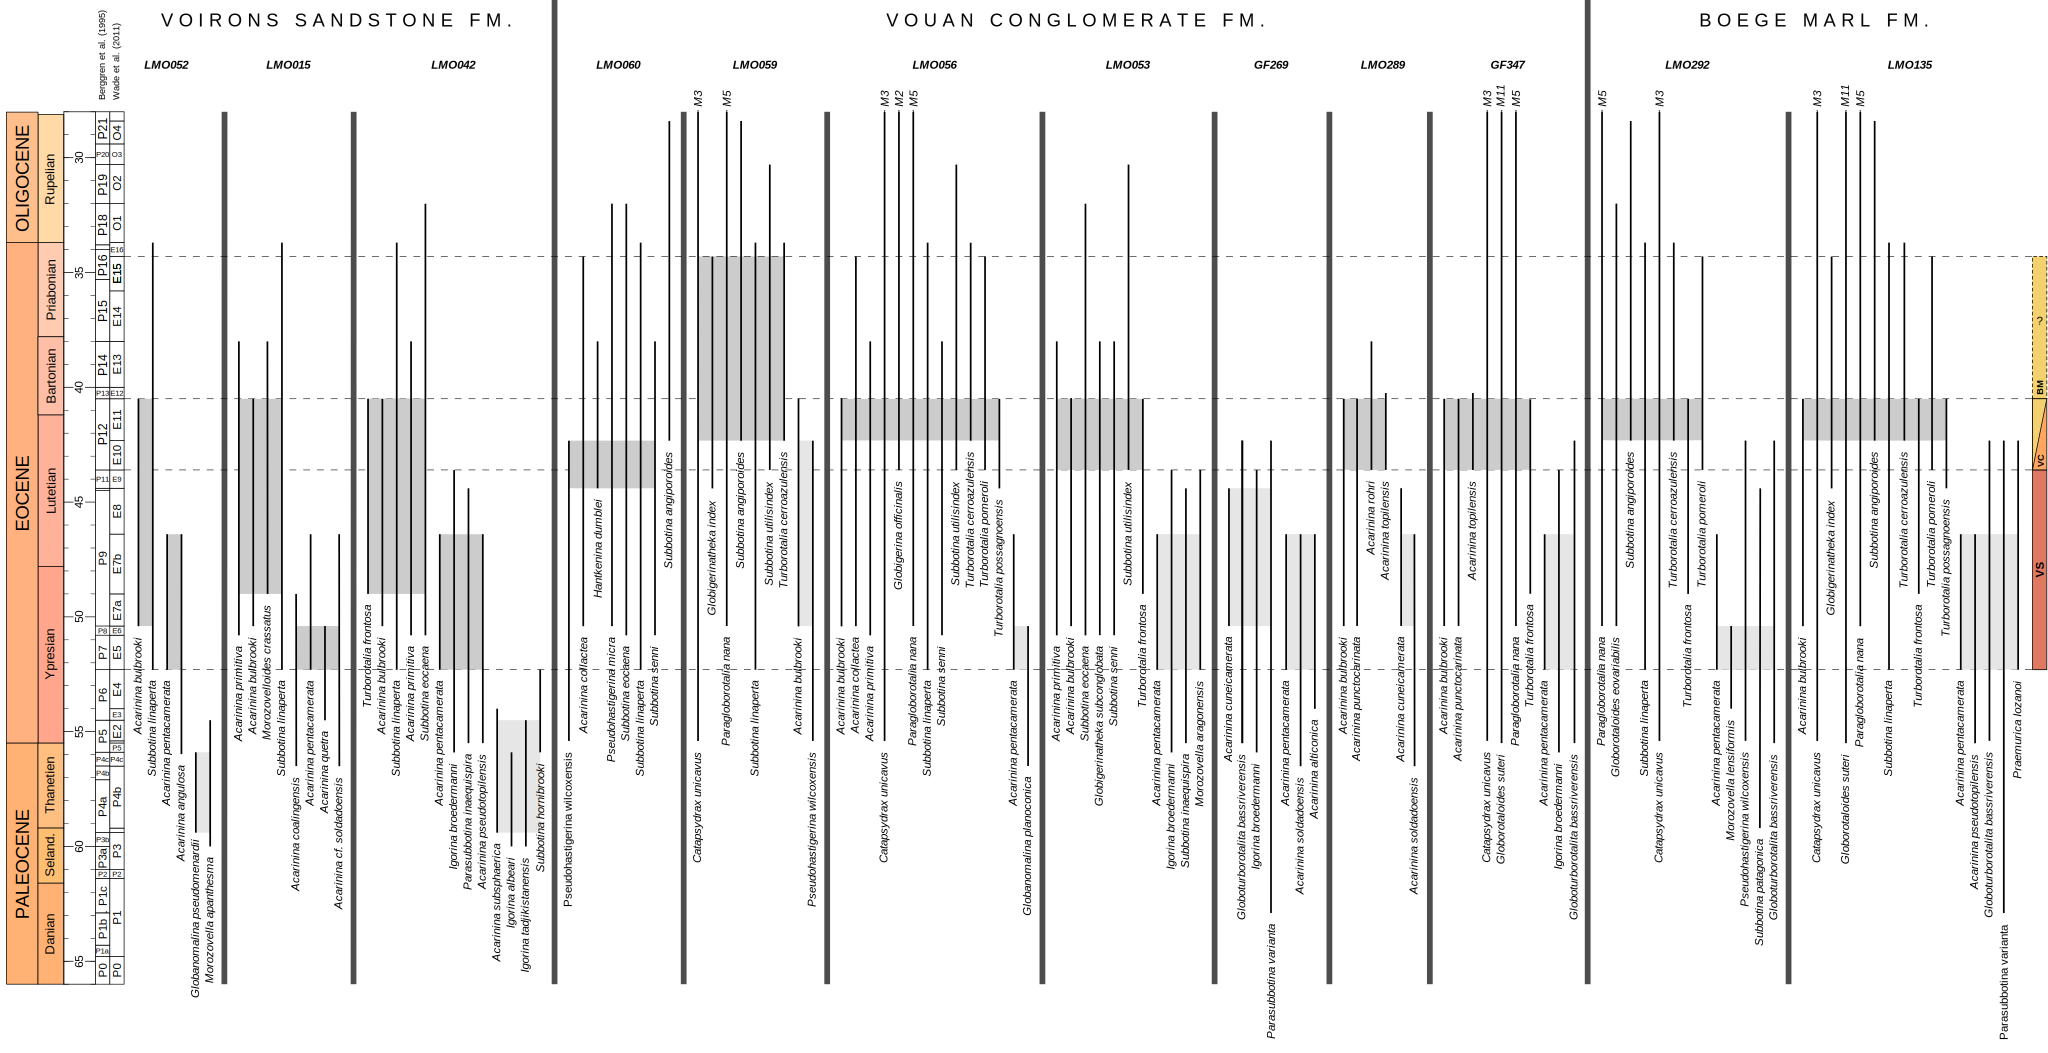
\includegraphics[width=\textwidth]{Fig5.pdf}
		\caption{Main studied outcrops: (a) the Bons quarry (VS), (b) the lower Saxel quarry (VS), (c) the Vachat millstone quarry (VC), (d) the Chauffemérande creek (BM), (e) The Grotte aux Loups (VC), (f) the Fenalet quarry (UH ?), (g) the Fayaux quarry (Fayaux-Pléiades Flysch) and (h) the Zollhaus quarry (Berra-Schwyberg Flysch). Location map is available in Figures~\ref{fig:Fig1} and~\ref{fig:Fig3}.}
		\label{fig:Fig5}
	\end{figure}
	}

\afterpage{
	\begin{figure}[htp!]
		\centering
		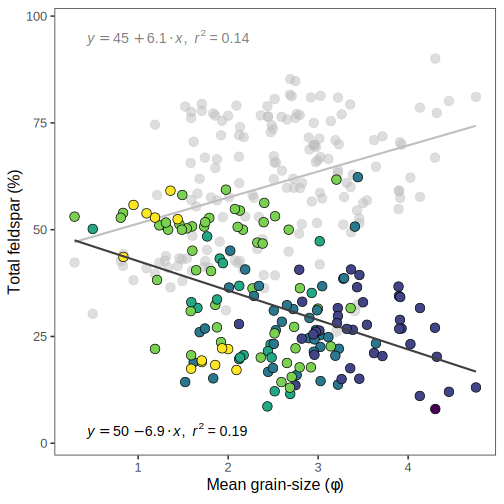
\includegraphics[width=\textwidth]{Fig6.pdf}
		\caption{Microphotography and macrophotography of typical grains found in the Voirons Flysch: (a) pink granite fragment, (b) black Paleozoic sandstone fragment, (c) mudstone fragments, (d) foraminifera and bioclastic wackestone fragment, (e) siliciclastic wackestone, bioturbation filling ?, (f) phosphatized foraminifera, (g) metamorphic clasts with micaceous lineations, and (h) tectonized quartz polycrystalline grains. The black bar represents \SI{200}{\micro\meter}.}
		\label{fig:Fig6}
	\end{figure}
	}
	
\section{Methods}

\subsection{Sampling}

Total amount of 278 sandstone samples was collected in about fifty outcrops of the Voirons Flysch. An additional exposure, the Fenalet quarry (Fig. 5f), to the East of the Allinges Hills, was also investigated, although it is generally attributed to the Ultrahelvetic because of its structural position and age \citep{Gagnebin1944,Badoux1962a,Badoux1965b,Badoux1996}. The Fayaux (Fig. 5g; \citealp{Stuijvenberg1976}) and the Zollhaus quarries (Fig. 5h; \citealp{Bouma1962,Crimes1981}), that comprise respectively the Fayaux-Pléiades and the Berra flyschs, were also sampled for comparative purposes. Geographic location of the outcrops, stratigraphic logs and datasets are available on the GitHub page of the first author (\url{https://github.com/jragusa/}).

\subsection{Thin-section modal mineralogy}

Counting was performed according to the Gazzi-Dickinson method \citep{Dickinson1979a,Ingersoll1979,Dickinson1985}. Grains were organised following the Zuffa classification \citep{Zuffa1980}. 300 extrabasinal grains was counted per thin section using the ribbon method of \cite{VanderPlas1962}. Feldspar minerals were stained following the procedure developed by \cite{Norman1974} and advices from Prof. Wilfried Winkler (ETH-Z\"urich). Using this technique, albite remains colourless but, in contrast to quartz grains, it is etched along the cleavage planes. Grains included in rock fragments (quartz, feldspars and micas) were counted separately \citep{Critelli2007,Stefani2007,DasGupta2008} and described according to the nomenclature of \cite{Weltje2002} (--rv: volcanic rock, --rm: metamorphic rock, --rg: plutonic rock). Sand-size quartz and feldspars from igneous rock fragments are reported in their respective QAP ternary diagram (Quartz -- Alkali feldspar -- Plagioclase). By convention, we distinguished lithic fragments (i.e. polycrystalline grains with internal grain-size less than \SI{63}{\micro\meter}) from rock fragments (internal grain-size coarser than \SI{63}{\micro\meter}). Metamorphic lithic and rock fragments were determined following the colour guide of \cite{Garzanti2003}. They are distributed between the low- (Rm1+), intermediate- (Rm3+) and high-metamorphic (Rm5+) grades, and described using the MI index (Metamorphic Index: \citealp{Garzanti2004,Garzanti2010}. Considering the sand-size limit, metamorphic grains of grade five were counted as rock fragments (Rm5). The status of mudstone and wackestone lithoclasts (Figs. 6c and 6d) is still questionable as there is no undisputable evidence for an extrabasinal origin \citep{Zuffa1980}. They can be inherited from a sedimentary cover (extrabasinal origin) or reworked from a platform (intrabasinal origin; \citealp{Critelli2007}). In addition, the incorporation of calcareous grains in the counting is debated \citep{Dickinson1979a,Mack1984}. Calcareous grains are very sensitive to weathering and a small amount of terrestrial calcareous grains reaches marine basins \citep{Arribas2000,Picard2007}. Considering that inclusion of detrital carbonate grains confers consistent provenance interpretation in some cases \citep{Mack1984}, our results are presented without (continuous line) and with (dashed line) the micritic limestone clasts. In addition, grain counting includes also intrabasinal grains (authigenic and skeletal grains), cement and porosity.\par
\medskip
Because formation boundaries are poorly defined in the Voirons Flysch \citep{Stuijvenberg1980a,Stuijvenberg1980b,Vial1989,Coppo1999}, the framework composition of samples was sorted independently of stratigraphic affiliation using a cluster analysis (Ward method and Euclidean distance; Fig. 7). Only grain classes exceeding 10~\% were selected (Qm, K, Lm, Qr, P, Ls, Lce, Qp, Lv and Lci; see Table 1 for description) to constrain the interpretation of the cluster tree, and limit the influence of minor grain classes. Each cluster defines a petrofacies which refers to similar compositional parameters \citep{Dickinson1972}.

\afterpage{
	\begin{figure}[htp!]
		\centering
		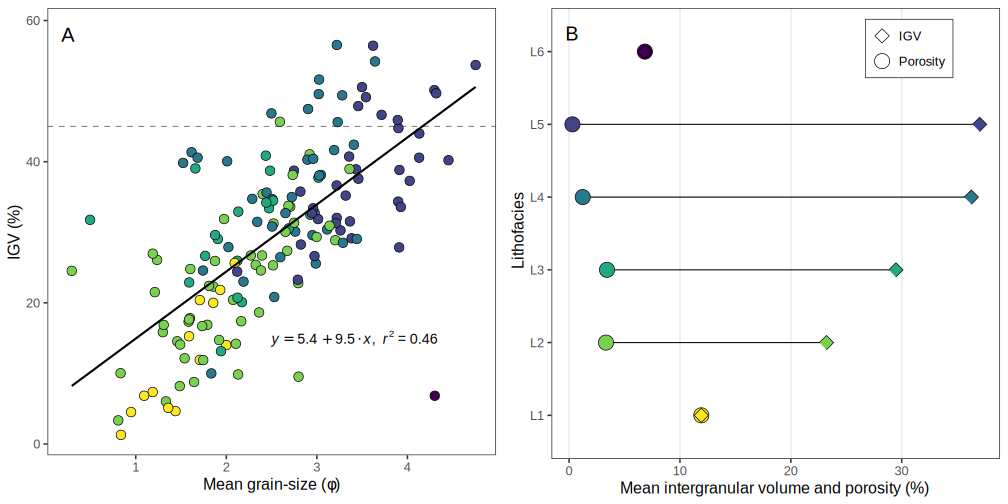
\includegraphics[width=0.5\textwidth]{Fig7.pdf}
		\caption{a) Relative proportion of the petrofacies within each stratigraphic unit. AS: Allinges Sandstone, BM: Boëge Marl Fm., Gu: Other flyschs of the Gurnigel nappe, UH: Fenalet quarry (Ultrahelvetic ?), VC: Vouan Conglomerate Fm., VS: Voirons Sandstone Fm. b) Cluster tree diagram with the two identified petrofacies.}
		\label{fig:Fig7}
	\end{figure}
	}
	
\afterpage{
	\begin{figure}[htp!]
		\centering
		
\includegraphics[width=0.5\textwidth]{Fig8.pdf}
		\caption{Box-whisker plot of the main grain classes of \cite{Zuffa1980}.}
		\label{fig:Fig8}
	\end{figure}
	}

\subsection{QEMSCAN heavy mineral analyses}

Heavy mineral were sampled from each petrofacies identified from the framework composition. They were extracted from fine- to medium-grained, well-preserved sandstones following \cite{Mange1992}. The rocks were crushed and cement removed with acetic acid (10~\%) in a hot bath (70°C). The \SIrange{63}{125}{\micro\meter} fraction of loose sediment was recovered by wet sieving. Dense minerals were separated using a liquor of sodium polytungstate (SPT) at d = 2.90 g/cm3, and recovered by freezing the bottom part of centrifugation tube. Heavy and light mineral fractions were then dried and weighted. Finally, the heavy mineral fraction was placed in moulds, consolidated with an epoxy resin, and subsequently polished to be analysed by an FEI QEMSCAN\registred\ Quanta 650F installed at the Department of Earth Sciences of the University of Geneva.\par
\medskip
The QEMSCAN\registred\ mineral phase identification relied on the combination of back-scattered electron (BSE) contrast and EDS spectra giving information on the elemental composition \citep{Gottlieb2000}. Individual X-ray spectra were compared to a library of known spectra and a mineral name was assigned to each individual acquisition point. The X-ray EDS spectra library, initially provided by the manufacturer, has been further developed in-house using a variety of natural standards. Measurements were performed on carbon-coated plugs that were adequately polished. Analytical conditions included a high vacuum and an acceleration voltage of 25 kV with probe current of 10 nA. The X-ray acquisition time was 10 ms per pixel using a point-spacing of 5 µm. Up to 122 individual fields of view were measured in each sample, with 1.5 mm per single field. QEMSCAN\registred\ data processing (e.g. unknown spectra debugging, particle boundary disambiguates, field stitching) was performed using the FEI iDiscover software. Composite mineral entries like garnet and tourmaline were defined by their respective EDS spectra consisted of individual elemental peak. Their intensities are defined by the ratios of measured elemental peaks and theoretical peaks representing a single pure compounds matter solely consisted of the element in question. Henceforth, the garnet entry comprises a comprehensive chemistry covering most of garnet species. Such a mean composition is defined by the following peak intensities: 35-200 (oxygen), 50-140 (aluminium), 80-210 (silicon), 20-210 (iron), 0-140 (magnesium), 0-100 (calcium) and Al/Si ratio that exceeded 0.3. Following the analogue reasoning the tourmaline composition used in this research consisted of oxygen (variable intensities), aluminium (140-280), silicon (120-220), sodium (0-45), magnesium (0-104), calcium (0-38), and iron (0-200), whereas fluorine and carbon may be encountered in EDS spectrum fitting the tourmaline entry compositional criteria.
Garnet grains are organised into six different classes including melting phases: almandine, almandine-pyrope, almandine-pyrope-grossular, almandine-spessartine, grossular and undetermined garnets. Tourmaline grains are grouped into schorl, dravite and undetermined tourmaline. For each mineral group, the elemental composition of ten grains is extracted within each class and for each sample.
In addition, 595 and 255 representative grains of garnet and tourmaline respectively were analysed by SEM-EDS system using an FEI QEMSCAN\registred\ Quanta 650F installed at the Department of Earth Sciences of the University of Geneva that was operated in the scanning electron microscope mode. The Bruker ESPRIT software was used for EDS spectra quantification in a standardless mode. Thereafter, garnet and tourmaline phase chemistry served as a basis to calculate the proportions of end-members of respective minerals using the spreadsheets designed by Andy Tindle from the Open University of Buckinghamshire for garnet (\url{http://www.open.ac.uk/earth-research/tindle/AGTWebPages/AGTSoft.html}).\par
\medskip
The HMC (Heavy Mineral Content) and tHMC (transparent Heavy Mineral Content) indices of \cite{Garzanti2007a} provide the heavy mineral content in sandstone. They are based on the improved estimation of the H index of \cite{Baker1962}. A preliminary single garnet grain analysis was performed by QEMSCAN\registred\. The different species of the garnet supergroup \cite{Grew2013} detected by QEMSCAN\registred\ are constrained to the most abundant species, the transitional solid-solution members and an undetermined group which gathers all the species are not documented in QEMSCAN\registred\ database.

\subsection{Thin section heavy mineral counting}

Ten heavy mineral fractions (\SIrange{63}{400}{\micro\meter}) from \cite{Ragusa2009} were also recounted (Table 3). The protocol extraction is similar to those of the QEMSCAN\registred\ analysis, apart of the use of bromoform (d = 2.89 g/cm3) and the recovering by filtration. Thereupon, heavy mineral fractions were dried and placed on thin section. Total amount of 200 transparent heavy mineral grains was counted.

\subsection{Data processing}

Mineral abbreviations are based on the compilation of \cite{Whitney2010} with a few exceptions like limonite (= Lim) to avoid confusion with metamorphic lithics (Lm). Additional grains are reported in Table 1. Computations and statistical analysis were performed using the R software \citep{RCoreTeam2015}. Samples distribution in a ternary diagram (Figs 9, 11, 17 and 19) is associated with fields indicating 90~\% confidence regions for the distribution, calculated via Mahalanobis Distance and Log-Ratio transformation \citep{Hamilton2016}, which is more accurate and reliable \citep{Weltje2002} than a hexagonal confidence area \citep{Ingersoll1978}. QEMSCAN\registred\ results were treated in FEI iDiscovery software v.5.2.

\section{Results}

\subsection{Voirons Flysch framework composition}

The dataset of the modal mineralogy of the Voirons Flysch is attached in supplementary data (Table A1). It describes raw data and stratigraphic affiliation for each sample. Samples are composed of poorly to well-cemented sandstones (Fig. 8). Sandstone beds mostly contain non-carbonate extrabasinal grains (NCE, 27.0 - 97.5~\%), minor carbonate intrabasinal grains (CI, 0 - 11.13~\%) and non-carbonate intrabasinal grains (NCI, 0 - 18.54~\%). Cl grains comprise a typical heterozoan assemblage including, in decreasing order, red-algae, foraminifers (e.g. nummulitids, discocyclinids, planktonic foraminifera), bryozoan and echinoid fragments, whereas the NCI grains consist of glauconite, phosphates (single grains and recrystallised foraminifers, Fig. 6e) and of some opaque minerals. Mudstone to wackestone lithoclasts were incorporated into the CI class, and consequently the proportion of carbonate extrabasinal (CE) grains is very low (< 2.5~\%). Calcite cement mostly fills up interstitial voids (0 – 63.3~\%) and porosity is usually very low, but may reach up to 25.6~\% in few cases.\par
\medskip
Cluster analysis on framework composition identifies two branches of different importance (Fig. 7). Based on their framework composition, the right branch (75.90~\% of the samples) is determined as a Quartzose petrofacies, whereas the left branch (24.10~\% of the samples) corresponds to a Feldspathic petrofacies. The Quartzose and Feldspathic petrofacies are mainly identified by distinctive Qm/F ratio (Figs. 9 and 10) with a slight overlap of the confidence areas. The incorporation of polycrystalline quartz (Qp) into the Q pole of the QFL diagram (Fig. 9a) emphasises their important proportion, flattening the scatter plot along the Q–F axis.

\afterpage{
	\begin{figure}[htp!]
		\centering
		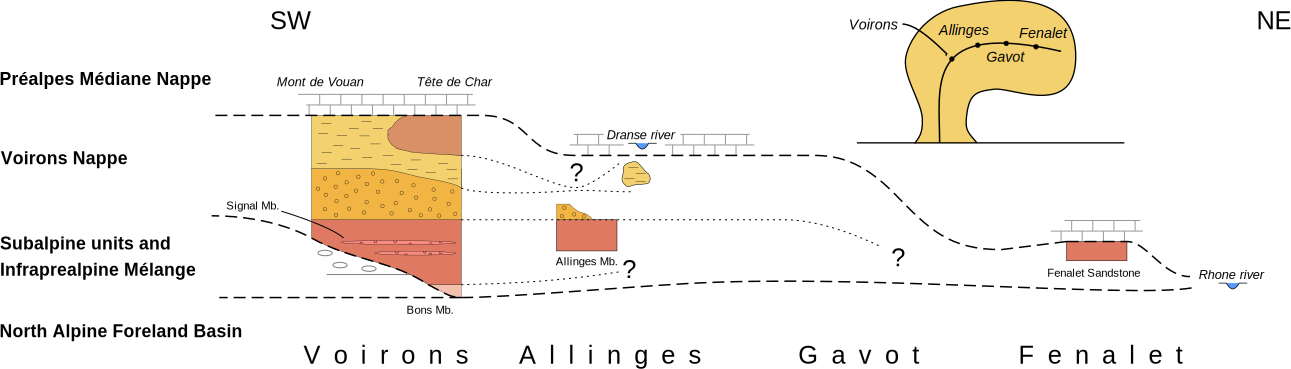
\includegraphics[width=0.75\textwidth]{Fig9.pdf}
		\caption{Petrofacies distribution in the QFL and QmFLt ternary diagrams of the Dickinson model.}
		\label{fig:Fig9}
	\end{figure}
	}

\subsubsection{The Quartzose petrofacies}

The Quartzose petrofacies presents a high Q/F ratio (Fig.~\ref{fig:Fig10}). The incorporation of mudstone to wackestone lithoclasts in the counting, especially in the QFL ternary diagram (Fig. 9a), reduces the strong influence of polycrystalline quartz in the samples of the Quartzose petrofacies. Considering the low lithic content and regarding the overall composition, the relative contribution of these micritic grains is low (Lc/QFL ratio, Fig.~\ref{fig:Fig10}), which explains the similar distribution in the QmFLt ternary diagram (Fig.~\ref{fig:Fig9}b).\par
\medskip
The distribution of monocrystalline grains (Fig.~\ref{fig:Fig11}a) shows a Qm–KP trend without a clear distinction within feldspars. The sample distribution is similar to that on QFL and QmFLt diagrams (Fig.~\ref{fig:Fig9}), emphasising the strong influence of the Q/F ratio in the petrofacies. The distribution of quartz is shown in the ternary diagram QmsQpQr (Fig.~\ref{fig:Fig11}b). Samples are concentrated around the Qm pole drawing a trend toward the Qr pole. The latter is mostly represented by a granitic source (Qrg/Qr ratio, Fig.~\ref{fig:Fig10}) The Quartzose petrofacies is mature with a high proportion of monocrystalline quartz. The proportion of polycrystalline quartz is very low (Qp/Q ratio, Fig.~\ref{fig:Fig10}), and the discrimination of the provenance is not as pronounced as in QFL (Fig.~\ref{fig:Fig9}) and QpLsmLvm ternary diagrams (Fig.~\ref{fig:Fig11}a). The composition of feldspar grains ranges from orthoclase to anorthite with a low albite content (Fig.~\ref{fig:Fig11}c). However, a slight increase in the albite content, together with the alkali-feldspars, can be explained by the relative depletion of calcium plagioclase by albitisation, as already pointed out by \cite{Morad1990}. Single grains represent the most abundant feldspars grains (Figs.~\ref{fig:Fig11}d and~\ref{fig:Fig11}e).\par
\medskip

\afterpage{
	\begin{figure}[htp!]
		\centering
		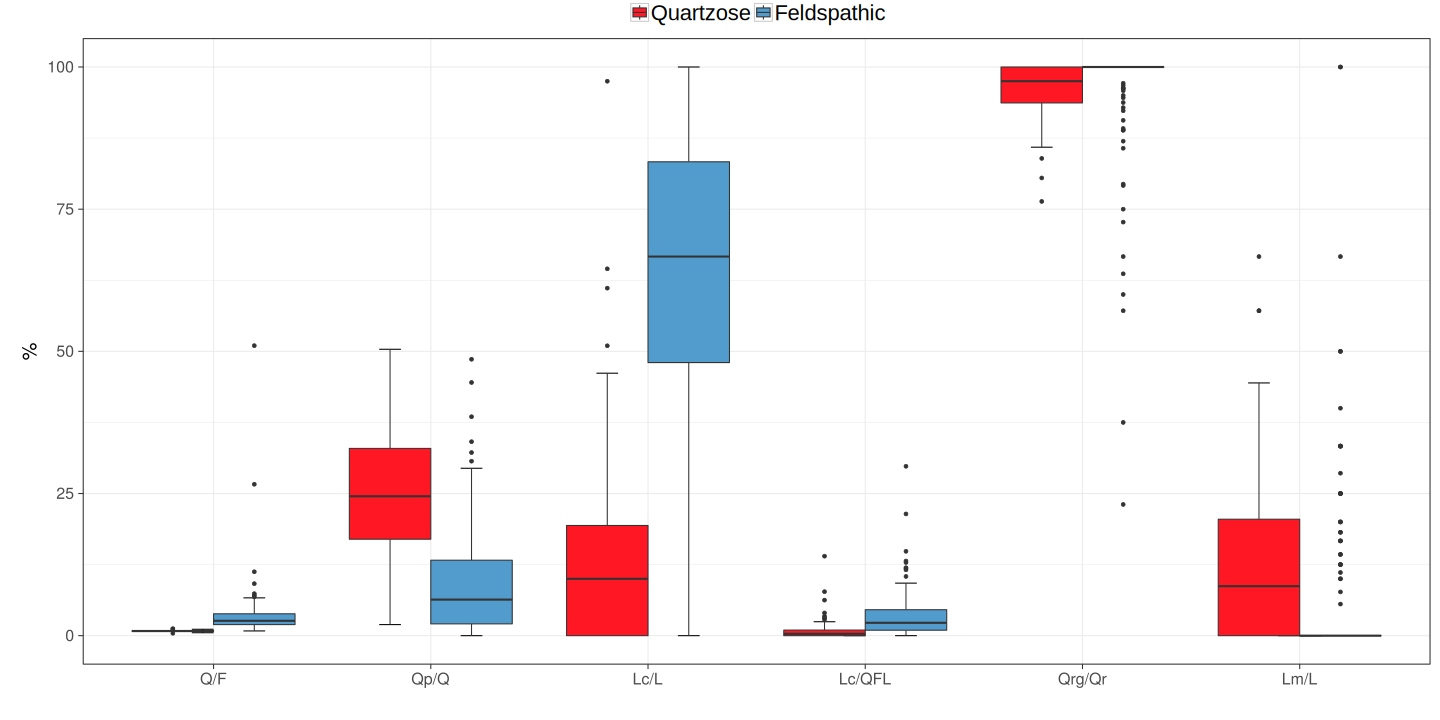
\includegraphics[width=0.75\textwidth]{Fig10.pdf}
		\caption{Box-whisker plot of the main ratio for the framework composition. For key to box plots see Fig.~\ref{fig:Fig8}.}
		\label{fig:Fig10}
	\end{figure}
	}

\afterpage{
	\begin{figure}[htp!]
		\centering
		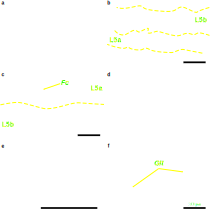
\includegraphics[width=\textwidth]{Fig11.pdf}
		\caption{Monocrystalline grain distribution illustrated with overall composition (a) and dedicated distribution of quartz (b) and feldspars (c to e). Polycrystalline grain distribution illustrated with overall composition (f and g), estimated composition of plutonic (h), volcanic rocks (i) and metamorphic grades of Garzanti et al. (2004) (j). Metamorphic inputs are also evaluated with the the MI index (Garzanti et al., 2004; Garzanti et al., 2010) (k) and the relative content of tectonic polycrysalline quartz (l).}
		\label{fig:Fig11}
	\end{figure}
	}

Several samples of the Quartzose petrofacies are devoid of lithic grains, and thus cannot be used in the analyses (L = 0, Fig.~\ref{fig:Fig10}). The distribution of lithic fragments identifies a magmato-sedimentary assemblage (Fig.~\ref{fig:Fig11}d). However, the lithic grains are subordinate to the high content of polycrystalline quartz, as illustrated in the QpLsmLvm ternary diagram (Fig.~\ref{fig:Fig11}e).
The inclusion of mudstone to wackestone grains confers a more sedimentary-rich composition to the Quartzose petrofacies (Lc/L, Fig.~\ref{fig:Fig10}). Sedimentary clasts are mostly represented by intrabasinal micritic limestone grains (Lcmi) presenting a large spectrum of textures from mudstones (Fig.~\ref{fig:Fig6}c) to foraminifer- and bioclast-rich wackestones (Fig.~\ref{fig:Fig6}d). The grain shapes are variable, from rounded to angular. Some micritic grains presenting a fuzzy boundary and containing quartz and glauconite (Fig.~\ref{fig:Fig6}e) could possibly correspond to the filling of bioturbations. The lack of oxidised contours or other post-sedimentary weathering features \citep{Zuffa1980} precludes an extrabasinal origin for these grains which are included in the CI grains as rip-up clasts reworked from the platform \citep{Garzanti1991}. Others sedimentary grains include chert debris, silt-size argillaceous fragments, and very rare recrystallised limestone clasts. The chemical and mechanical stability of chert fragments facilitates their persistence in the sedimentary record, which leads to overestimate their relative content. They could be an indicator of carbonate source rocks \citep{Mack1984}. Clayey to silty fragments are undoubtedly extrabasinal, but do not provide any information about their respective source. Sandstone fragments are usually absent as they directly provide single grains (e.g. quartz, feldspars). By contrast, conglomerate fragments were found in the conglomerate layers. Amber grains have been reported in the Allinges Sandstone \citep{deMortillet1863,Renevier1893b} and in the Vouan Conglomerate Fm. \citep{Pilloud1936}. Sparse phosphate grains and phosphatised foraminifers are also found (Fig.~\ref{fig:Fig6}g), especially in the Boëge Marl Fm. No trend can be deduced from the sedimentary clasts as their distribution varies strongly through the samples. The relative content of the CE grains in sandstone samples is very low (Fig.~\ref{fig:Fig8}), which contrasts to their widespread occurrence in conglomerates \citep{Cogulu1961,Winkler1983,Frebourg2006}). This may result either from (1) preferential dissolution, (2) late incorporation in the sedimentary process or (3) dilution by comparatively better-preserved igneous rocks.\par
\medskip
Magmatic clasts are both of plutonic and volcanic origin. Most of the examined grains are plutonic rock-fragments (Fig. 11f), and plot in the granite to granodiorite fields, extending up to the tonalite field in some samples. Some microgranites were also encountered. The low proportion of volcanic grains precludes a reliable identification of volcanic-rock fragments. Samples plot in the quartz andesite to rhyolite fields (Fig.~\ref{fig:Fig11}g), and andesitic lithoclasts have been reported in thin sections \citep{Ospina-Ostios2013}.\par
\medskip
The Quartzose petrofacies is usually devoid of metamorphic grains (Lm/L ratio, Fig.~\ref{fig:Fig10}). Thus, few points are plotted inside the ternary diagrams (Fig. 11h). They are concentrated near the end members or along the axis due to their scarcity. However, considering the mean values, the Quartzose petrofacies is preferentially located near the Rm5+ end member (High metamorphic grade). The Metamorphic index is low (Figs.~\ref{fig:Fig10} and ~\ref{fig:Fig11}i), and the Quartzose petrofacies presents also a low amount of tectonised polycrystalline quartz (Figs.~\ref{fig:Fig10} and ~\ref{fig:Fig11}j) which is typical of remnant oceanic deposits off- scraped at shallow levels \citep{Garzanti2010}.

\subsubsection{The Feldspathic petrofacies}

The Feldspathic petrofacies presents a low Q/F ratio (Fig.~\ref{fig:Fig10}). Samples are not affected by the counting of mudstone to wackestone fragments (Fig. 8), which emphasises the scarcity of these grains in this provenance (Lc/L ratio, Fig.~\ref{fig:Fig10}).\par
\medskip
The Feldspathic petrofacies shows a high content in plagioclase among monocrystalline grains (Fig.~\ref{fig:Fig11}a). Some albitisation of plagioclase \citep{Morad2000} is also observed as suggested by the minor content in albite (Fig.~\ref{fig:Fig11}c). Quartz grains comprise an elevated content in lithic quartz grains (Fig.~\ref{fig:Fig11}b, Qr) and polycrystalline quartz (Qp/Q ratio, Fig.~\ref{fig:Fig10}). The latter usually originate from granitic rock fragments (Qrg/Qr ratio, Fig.~\ref{fig:Fig10}), but gneisses cannot be excluded as an alternative source of polycrystalline quartz.\par
\medskip
The Feldspathic petrofacies always contains a significant fraction of lithic fragments (Figs.~\ref{fig:Fig11}d and~\ref{fig:Fig11}e) including a large proportion of metamorphic lithoclasts (Lm/L ratio, Fig.~\ref{fig:Fig10}), in addition to the magmato-sedimentary assemblage. However, the lithic grains are less abundant than the polycrystalline quartz (Fig.~\ref{fig:Fig11}e), and the confidence areas present a large overlap with the Quartzose petrofacies (Figs.~\ref{fig:Fig11}d and~\ref{fig:Fig11}e).\par
\medskip
The magmatic lithic content is relatively similar to that described in the Quartzose petrofacies (Figs.~\ref{fig:Fig11}f and~\ref{fig:Fig11}g). Sample distribution overlaps the Quartzose petrofacies in the plutonic rocks (Fig.~\ref{fig:Fig11}f). More volcanic rocks are observed in the Feldspathic petrofacies and plot in the Rhyodacite to Quartz-andesite fields (Fig.~\ref{fig:Fig11}d). The Feldspathic petrofacies is characterised by significant inputs in metamorphic rock fragments (Lm/L ratio, Fig.~\ref{fig:Fig10}) and a high MI index (Figs.~\ref{fig:Fig10} and~\ref{fig:Fig11}i) dominated by high-grade, with subordinate low-grade, metamorphic lithics (Figs.~\ref{fig:Fig11}i and~\ref{fig:Fig11}j). However, such a high MI value is not common in remnant-ocean deposits off-scraped at shallow depth (Garzanti et al., 2010; Fig.~\ref{fig:Fig8}). Protoliths likely consist of sedimentary rocks according to the nomenclature of \citep{Garzanti2003}. Tectonised polycrystalline quartz (QpT) stands for a reliable indicator of the supply of metamorphic rock fragments (\citealp{Young1976}; Figs.~\ref{fig:Fig10} and~\ref{fig:Fig11}j). The metamorphic clasts, especially schists, are more easily crushed during the sediment transport \cite{Picard2007}.

\subsection{Voirons Flysch heavy-mineral assemblage}

The dataset of the heavy minerals of the Voirons Flysch is summarised in Table 2 and Table 3 for the QEMSCAN\registred\ analyses and the samples from \cite{Ragusa2009} respectively. The abundance of heavy minerals and transparent heavy minerals (HMC and tHMC) in the \SIrange{63}{125}{\micro\meter} fraction is poor to moderately poor (sensu \citealp{Garzanti2010}) in both petrofacies (Fig. 12; Table 2). The small gap between HMC and tHMC indices illustrates an elevated content of transparent heavy minerals (tHM). The assemblage of tHM represents 60 to 90~\% of the dense minerals followed by opaque grains and micas \citep{Ragusa2015}. The lowest content in tHM is found in the distal density-current deposits (JR5 and JR57), and is associated with a higher mica content (Fig. 13). In both grain-size range, transparent heavy minerals are represented by ultrastable (ZTR group) and stable (garnet and apatite) species in both petrofacies (Fig. 14). Accessory grains of the tHM trace group consist of unstable minerals (e.g. barite, epidote, pyroxene and hornblende).\par
There is some discrepancies between the both fractions. The main difference lies in the relative distribution of the mineral species (e.g. higher zircon and lower rutile content in the 63-400 µm). Rutile and titanite are relatively more abundant in the \SIrange{63}{125}{\micro\meter} fraction than staurolite, tourmaline and zircon and inversely in the \SIrange{63}{400}{\micro\meter} fraction. These differences may derive from inherited grain-size in source rocks \citep{Morton1999}. In addition, the QEMSCAN\registred\ determination may also influence the relative proportion with a better identification of the finest fraction which is more difficult to constrain with an optical microscope. Despite these discrepancies, the relative abundance of some diagnostic species (e.g. garnet), or dedicated ratios discriminate Quartzose and Feldspathic petrofacies in both grain-size ranges (Figs. 12 and 14).

\afterpage{
	\begin{figure}[htp!]
		\centering
		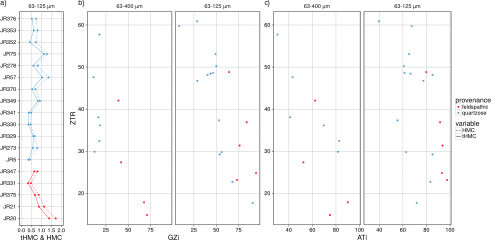
\includegraphics[width=\textwidth]{Fig12.pdf}
		\caption{Heavy mineral indices. (a) tHMC: transparent heavy mineral content \citep{Garzanti2007a}, (b) ZTR versus GZi (garnet/garnet+zircon) and (c) ZTR versus ATi (apatite/apatite+tourmaline) from \cite{Morton1994}}
		\label{fig:Fig12}
	\end{figure}
	}
\afterpage{
	\begin{figure}[htp!]
		\centering
		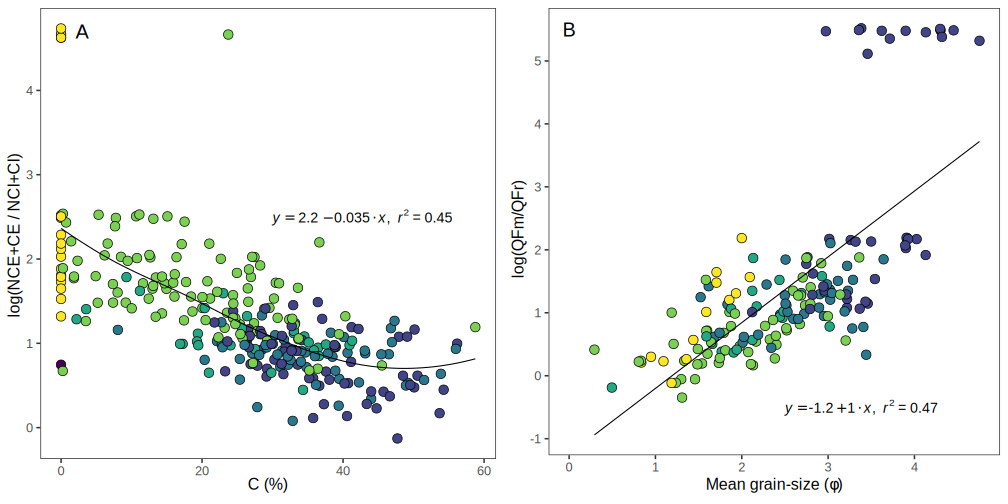
\includegraphics[width=0.5\textwidth]{Fig13.pdf}
		\caption{Mica distribution in the \SIrange{63}{125}{\micro\meter} fraction}
		\label{fig:Fig13}
	\end{figure}
	}
\afterpage{
	\begin{figure}[htp!]
		\centering
		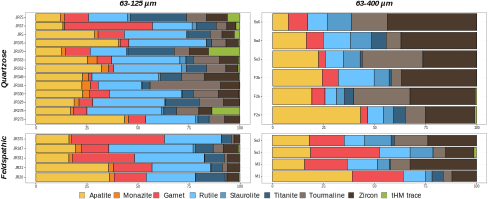
\includegraphics[width=\textwidth]{Fig14.pdf}
		\caption{Transparent heavy-mineral distribution for the \SIrange{63}{125}{\micro\meter} and recounted \SIrange{63}{400}{\micro\meter} fractions}
		\label{fig:Fig14}
	\end{figure}
	}
	
\subsubsection{The Quartzose petrofacies}

The Quartzose petrofacies essentially contains abundant tourmaline reflected by lower ATi \citep{Morton1994} and higher ZTR indices (Fig. 12; Table 2). The garnet content is low, as emphasised by the low GZi index (Fig. 12; Table 2; \citealp{Morton1994}). The scarce K-rich volcanic glass confirms the rhyolitic source described in Fig. 11g. A large variation in mica distribution and the occurrence of biotite characterise the Quartzose petrofacies.\par
Preliminary single-grain analysis on garnets identified almandine and almandine-pyrope solid solution (mean = 86.09~\%) as dominant phases (Fig. 15a). Subordinate grains are almandine-pyrope-grossular and almandine-spessartine solid solutions (mean = 6.95~\%). Less than 10~\% of garnets grains were undetermined. Moreover, the Quartzose petrofacies shows the schorl-dominated assemblage among tourmaline grains (Fig. 16).

\afterpage{
	\begin{figure}[htp!]
		\centering
		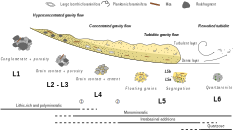
\includegraphics[width=\textwidth]{Fig15.pdf}
		\caption{Garnet geochemistry. \textbf{a} Relative distribution of the different classes identified by the QEMSCAN\registred, \textbf{b} ternary diagram of garnet discrimination after \cite{Mange2007a}, \textbf{c} SEM-EDS composition of the different garnet classes based on end-member abundances. For key to box plots see Fig.~\ref{fig:Fig8}}
		\label{fig:Fig15}
	\end{figure}
	}

\subsubsection{The Feldspathic petrofacies}

The Feldspathic petrofacies is characterised by a high content in garnet and an elevated GZi index in the \SIrange{63}{125}{\micro\meter} fraction (Fig. 12, Table 2). Consequently, the ATi index is high and the ZTR index is low (Fig. 12; Table 2). The distribution of micas is relatively constant in the Feldspathic petrofacies and is dominated by chlorite (Fig. 13). Single grain analysis on garnet identified almandine-pyrope-grossular and almandine-spessartine solid solutions, similar to the assemblages found in the Quartzose petrofacies. As for the latter, the tourmaline assemblage is dominated by schorl (Fig. 16).

\afterpage{
	\begin{figure}[htp!]
		\centering
		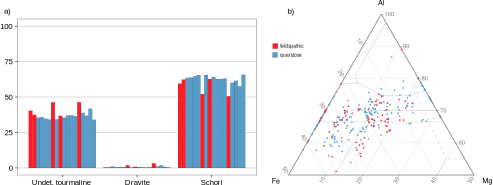
\includegraphics[width=\textwidth]{Fig16.pdf}
		\caption{Tourmaline geochemistry, a relative distribution of the different classes identified by the Q­EMSCAN\registred, b ternary diagram of tourmaline discrimination after \cite{Henry1985}}
		\label{fig:Fig16}
	\end{figure}
	}

\subsubsection{Garnet and tourmaline geochemistry}

The geochemical data of garnet and tourmaline are summarised in supplementary data (Tables A3 and A4 respectively). Both petrofacies share similar garnet distribution dominated by almandine (Alm) and almandine-pyrope (Alm-Prp) varieties (Fig. 15a). The relative composition of each class is summarised in Fig. 15c. Several classes contains a minor amount of andradite. The almandine-spessartine phase (Alm-Sps) includes a minor content in grossular. Undetermined garnets correspond to spessartine-almandine-grossular (Sps-Alm-Grs). Finally grossular (Grs) is relatively pure ($> 80~\%$) with few amount of andradite. Almandine-pyrope-grossular (Alp-Prp-Grs) is also reported in trace amount. Both petrofacies contain also a similar tourmaline composition dominated by schorl (Srl) and secondary dravite (Drv) (Fig 16). Undetermined tourmaline identified by the QEMSCAN\registred\ correspond to Drv-rich Srl. Tourmaline geochemistry shows a wide compositional variation governed by Fe content.

\section{Discussion}

\subsection{Petrofacies distribution in the stratigraphic subdivisions of the Voirons Flysch}

As mentioned previously, the stratigraphic units of the Voirons Flysch were up to now poorly differentiated from a petrographic viewpoint \citep{Lombard1940a,Stuijvenberg1980a,Charollais1998}. Our modal composition analysis demonstrates that the Vouan Conglomerate Fm. is restricted to the left branch of the cluster tree (Fig. 7), and shows a homogeneous composition (Fig. 9). It thus represents the most typical stratigraphic unit of the Feldspathic petrofacies. However, several samples from other formations, especially from the Voirons Sandstone Fm., are located on the same branch as the Vouan Conglomerate Fm. (Fig. 7). The feldspatho-quartzo-lithic composition of these samples strongly differs from the other samples of these formations, and rather corresponds to the Vouan Conglomerate Fm. They consist of single beds, randomly distributed in the Voirons Sandstone Fm., in the Boëge Marl Fm. and in the Bruant Sandstone Fm. (Fig. 17). They are numerous near the boundary between the Voirons Sandstone Fm. and the Vouan Conglomerate Fm. which suggests an interfingering rather than a tectonic contact between these two units (Fig. 17).
The other lithostratigraphic units of the Voirons Flysch are characterised by the Quartzose petrofacies (Fig. 7). The latter represents the major source of detritus of the Voirons Flysch, and presents a wide spectrum of composition controlled by the depositional settings in a deep-sea fan \citep{Ragusa2015}. The Quartzose petrofacies of the crest conglomerates (e.g. “Conglomérat de Pralaire”; \citealp{Lombard1940a}; Fig. 4) precludes an affiliation with the Vouan Conglomerate Fm., as stated by \citep{Stuijvenberg1980a}.\par
It is impossible to recognise the provenances from the observation of sandstone beds in the field, unless they are interstratified with conglomerate layers comprising typical lithoclasts (e.g. pink granite fragments for the Quartzose petrofacies and black sandstone clasts of Paleozoic age for the Feldspathic petrofacies). Hence, the localisation of the Feldspathic petrofacies in single beds of the Voirons Flysch and the fine-tuning of the boundaries of the Vouan Conglomerate Fm. remains problematic. In addition, these new data modify the stratigraphic affiliations of some outcrops \citep{Ragusa2015}. In particular, the framework composition of the deposits exposed in the Fenalet quarry indicates that they must be correlated with the Voirons Flysch, and not with the Ultrahelvetic units.

\afterpage{
	\begin{figure}[htp!]
		\centering
		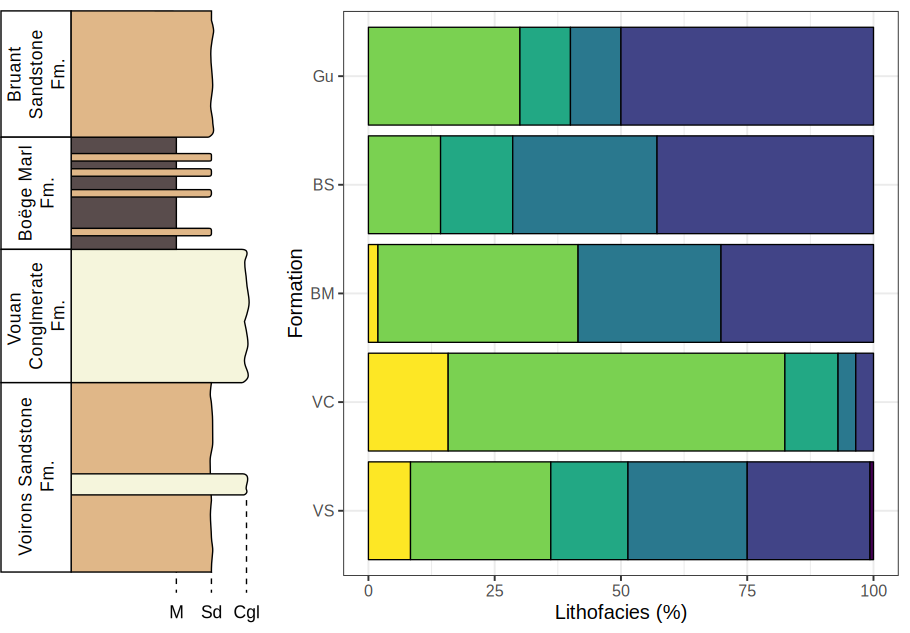
\includegraphics[width=\textwidth]{Fig17.pdf}
		\caption{Relationship between petrofacies and stratigraphic units illustrated by a synthetic log of the Voirons Flysch (\textbf{a}) and the QmFLt ternary diagram (Fig.~\ref{fig:Fig8}b) with the initial stratigraphic affiliation (\textbf{b}). Note the widespread location of most of the stratigraphic units}
		\label{fig:Fig17}
	\end{figure}
	}

\subsection{Provenance of the Quartzose petrofacies}

The quartz-rich composition and low HMC values of the Quartzose petrofacies correspond to the Transitional continental to Mixed tectonic settings (Fig. 9) of the Dickinson model \citep{Dickinson1985,Dickinson1979a}. Rock composition describes a low unroofed basement source including crystalline rocks and a sedimentary cover. The occurrences of zircon, tourmaline, xenotime, and monazite are common in intermediate to acidic granite and their metamorphic counterparts as well as in polycyclic detrital sandstones (Fig. 14; \citealp{Mange1992,Stefani2007,Eynatten2012}. Tonalite composition is confirmed by the high ATi index (Fig. 12; \citealp{Butler2011}) and the negative correlation of apatite with silicates \citep{Eynatten2012}. Occurrence of andesite grains has also been reported \citep{Ospina-Ostios2013}. Tourmaline grains plots in fields 2, 3, 4 and 5 of the ternary discrimination diagram (\citealp{Henry1985}; Fig. 16b), suggesting a wide range of source rocks. The latter include igneous rocks (fields 2 and 3) and metasedimentary rocks (fields 4 to 6) \cite{Henry1985,Mange1992}. In addition, the minor amount of dravite further suggests igneous rocks as the main source of tourmaline (Fig. 16a). Sedimentary inputs have probably been underestimated, and might contribute a lot to the detrital sedimentation \citep{Picard2007}. The ZTR index suggests an important reworking of detrital sedimentary rocks (Fig. 12). Sedimentary clasts found in conglomerate layers originate from a carbonate-rich stratigraphic succession of Triassic to Cretaceous age \citep{Ragusa2015}. Further analyses are needed to better constrain the source of some peculiar facies (e.g. neritic carbonates similar to Urgonian Limestones; \citealp{Lombard1940a}). Likewise, the widespread occurrence of phosphate in the Tethyan realm from the Cretaceous to the Eocene \citep{Broudoux1985,Notholt1989,Follmi1990} is not a reliable indicator of a palaeogeographic origin. Amber grains are also found in other locations of the Gurnigel nappe \citep{Tercier1928a}, and correspond to a fluvial or coastal source. They do not relate to a particular palaeogeographic origin.\par
Our petrographic data (quartz-rich assemblage, high ZTR index) further suggest that the Quartzose petrofacies is very mature, and experienced polycyclic sedimentation, as confirmed by its location in the Mixed field of the Dickinson model (Fig. 9). This may occur in a fluvial system by the migration of the river bed \citep{Amorosi2011} or in marine basins through the influence of an oceanic current \citep{Morton1999}. Likewise, the scattered presence of metamorphic fragments (Figs. 11h and 11i) could also result from the reworking of deposits related to the Feldspathic petrofacies. Following the Garzanti model \citep{Garzanti2007b}, the Quartzose petrofacies provenance can correspond either to the Continental block or to the Clastic wedge provenance.\par
Intrabasinal components, including chemical (glauconite and phosphate) and biological (bioclasts and micritic limestones) grains, are frequent in the samples from the Quartzose petrofacies. They indicate the reworking of platform sediments by gravity currents, especially during transgressive phases \citep{Odin1981,Garzanti1991}. A high amount of carbonate grains is characteristic of close-up basins \citep{Critelli2007}, and controls diagenetic processes such as cementation and porosity reduction (Fig. 18). The reworking of sediments could also be explained by the influence of marine currents \citep{Ingersoll1990,Ingersoll1993} especially during sea-level highstands \citep{Amorosi2011}. Hence, both allogenic and autogenic factors controlled the composition of the Quartzose petrofacies.

\afterpage{
	\begin{figure}[htp!]
		\centering
		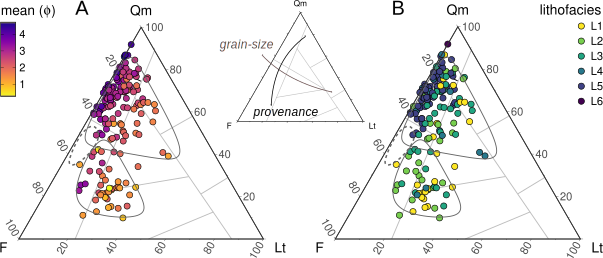
\includegraphics[width=0.5\textwidth]{Fig18.pdf}
		\caption{Relationship between extrabasinal vs. intrabasinal grains and cement vs. porosity}
		\label{fig:Fig18}
	\end{figure}
	}

\subsection{Provenance of the Feldspathic petrofacies}

The feldspar-dominated (Fig. 9) assemblage indicates a location in the Basement uplift to Dissected volcanic arc fields of the Dickinson model \citep{Dickinson1985,Dickinson1979a}. However, the source rocks are quite similar to those of the Quartzose petrofacies (Figs. 11 and 14). The main difference lies in the low sediment maturity in the Feldspathic petrofacies. Hence, it presents a lithic-rich composition (Figs. 9 and 11) with some andesitic and granitic rock fragments. The main characteristic of the Feldspathic petrofacies is the abundance of metamorphic lithics and rock fragments in sand-size grains (Fig. 11), and especially of the psammite-derived metamorphic lithics according to the colour guide of \citep{Garzanti2003}. Polycrystalline quartz (QpT) is a good indicator of these metamorphic inputs (Fig. 11d). The occurrence of staurolite (amphibolite facies), rutile (HP grade) (Fig. 14) and chlorite (low grade metamorphism) (Fig. 15) suggest a large variability of metamorphic rocks. They are presumably related to regional metamorphism and to low- to intermediate-grade meta-sediments \citep{Eynatten1999,Copjakova2005,Eynatten2012}. The association of garnet and staurolite may indicate a source in micaschist complexes \citep{Fuchtbauer1964}. According to the \citep{Mange2007a} garnet discrimination diagram (field Bi, Fig. 15b), the almandine-dominated garnet distribution (Alm and Alm-Prp) mostly corresponds to amphibolite-grade (MP-MT) metasedimentary rocks, thus corroborating the high metamorphic grade (Figs. 9e and 9f). The small amount of Alm-Sps and Sps-Alm-Grs could derive from granites and pegmatites or from metamorphic rocks such as higher greenschist facies (\citealp{Krippner2014}, field B Fig. 15b), whereas the scarce Grs may originate from contact metamorphosed marls or calcareous shale \citep{Win2007}. Besides, the low amount of pyrope precludes peridotite and eclogite source rocks \citep{Eynatten1999}.\par
The high amount of metamorphic grains correlates the Feldspathic petrofacies with the Axial belt provenance \citep{Garzanti2004,Garzanti2007b,Garzanti2010}. Such a provenance favours the entrainment of fresh material in the sedimentary cycle. However, the similarity with the Quartzose petrofacies strongly suggests that sediments of both petrofacies met comparable weathering conditions, regarding the scarcity of the other typical metamorphic unstable grains.\par
Intrabasinal grains (NCI and CI grains) are scarce in the Feldspathic petrofacies (Fig. 18) suggesting a reduced marine influence in the sand composition and a sparse cementation linked to the low carbonate content. Hence, allogenic factors, especially tectonics, controlled sediment composition of the Feldspathic petrofacies. This may explain the formation of this relatively unaltered proximal facies which is usually associated to sea-level lowstands \citep{Amorosi2011}.

\subsection{Regional comparison with the other Prealps flyschs}

Our data are compared with the following flysch deposits exposed in the Prealps (Figs. 1, 2 and 3): (1) the Upper Prealps flyschs \citep{Caron1972a,Fluck1973,Gasinski1997} represented by the Sarine, the Dranses and the Simme flyschs – South Penninic domain, (2) the Médianes Flysch \citep{Fluck1973,Caron1989} – Briançonnais domain, (3) the other flyschs from the Gurnigel nappe represented by the Schlieren \citep{Winkler1983,Winkler1984} and the Wägital flyschs \citep{Winkler1985b} and (4) the Niesen flyschs \citep{Ackermann1984,Ackermann1986} – Valais domain. The petrography of these units has been studied during the 1970-1980’s following the Gazzi-Dickinson method (Fig. 19), and salient results are compiled in \cite{Caron1989}.\par
\medskip

\afterpage{
	\begin{figure}[htp!]
		\centering
		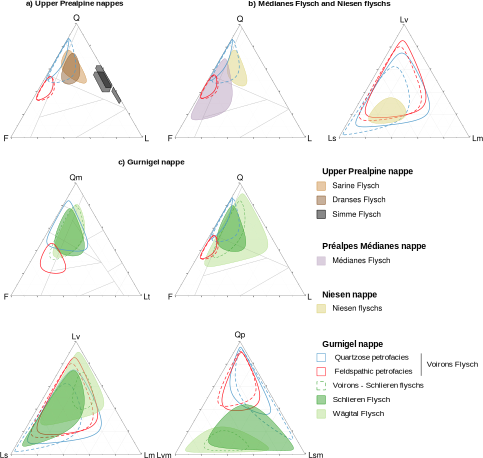
\includegraphics[width=\textwidth]{Fig19.pdf}
		\caption{Ternary diagrams of the Dickison model of the Voirons Flysch provenances compared to the Upper Prealps flyschs (\textbf{a}), the Médianes Flysch and the Niesen flyschs (\textbf{b}) and the other Gurnigel flyschs (\textbf{c}). See references in text}
		\label{fig:Fig19}
	\end{figure}
	}
\afterpage{
	\begin{figure}[htp!]
		\centering
		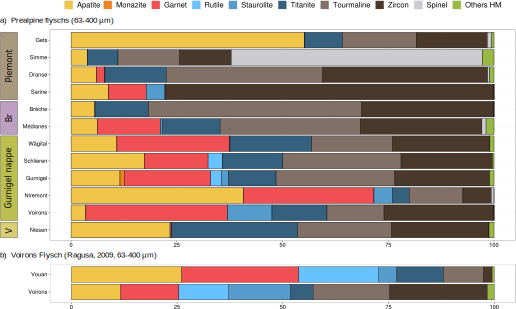
\includegraphics[width=\textwidth]{Fig20.pdf}
		\caption{Transparent heavy-mineral distribution in the Prealps flyschs (\textbf{a}) and mean distribution from the Voirons. Flysch with \SIrange{63}{125}{\micro\meter} and
\SIrange{63}{400}{\micro\meter} range \citep[modified]{Ragusa2009} (\textbf{b}). Br Briançonnais domain, V Valais domain. See references in text}
		\label{fig:Fig20}
	\end{figure}
	}

The first phase of flysch deposition in the Alps is represented by the Simme and the Gets flyschs. They are devoid of garnet grains, but contain a variable amount of chrome-spinel (Fig. 20a) which is inherited from the Piemont ophiolites \citep{Bertrand1976,Bill1997,Beltran-Trivino2013}. Their lithic-rich composition (Fig. 19a) emphasises massive inputs of fresh material from both continental and oceanic crusts \citep[and references therein]{Gasinski1997}. Framework composition describes a Recycled orogen tectonic setting \citep{Dickinson1979a} and an Ophiolite provenance \citep{Garzanti2007b}, considering the spinel-rich heavy minerals. They do not share any petrographic similarities with the flyschs from the Gurnigel nappe (Fig. 19a).\par
\medskip
The younger Sarine and Dranses flyschs have a similar framework composition characterised by a low lithic content (Fig. 19a). However, the heavy mineral populations are very different from the Simme and the Gets flyschs (Fig. 20a). The low garnet content indicates minor metamorphic inputs, whereas the high proportion of zircon and tourmaline indicates a granitic source. These flyschs plot in the Continental Block to Clastic wedge provenance according to the Garzanti model \citep{Garzanti2007b}. Their location in the Transitional continental to Mixed tectonic settings \citep{Dickinson1979a,Dickinson1985}, as well as the low garnet content, is similar to that of the Quartzose petrofacies (Fig. 19a).\par
\medskip
The composition of the Médianes Flysch is characterised by a feldspar-dominated composition. Garnet grains occur in the heavy-mineral assemblage of this flysch, but seems to be missing in the Brèche Flysch (Fig. 15) . The rare chrome-spinel grains found in the Médianes Flysch \citep{Fluck1973} are likely reworked from the Simme or the Gets flyschs \citep{Beltran-Trivino2013}. Provenance interpretation defines a Basement uplift tectonic setting \citep{Dickinson1979a,Dickinson1985}. The composition of the Médianes Flysch is very similar to the Feldspathic petrofacies of the Voirons Flysch, but is richer in lithic fragments (Fig. 14b). Scarce data from the Brèche Flysch precludes any provenance interpretation.\par
\medskip
The Schlieren and Wägital flyschs plot in the Transitional continental to Mixed fields of the Dickinson model. These units appear to differ from the Quartzose petrofacies because of the different interpretation of micritic lithoclasts and by a richer content in polycrystalline quartz. Incorporation of the micritic grains (Fig. 15c; dashed lines) in the counting provides similar results. The Wägital Flysch is characterised by an elevated content in metamorphic and volcanic lithoclasts. Garnet and staurolite contents are high, and equivalent to the zircon + tourmaline content. The Schlieren Flysch is rich in sedimentary lithoclasts, with the notable presence of dolostone fragments likely derived from Triassic deposits \citep{Winkler1983,Winkler1984}. Metamorphic inputs decrease, and the granitic source rather influences the heavy-mineral assemblage. Based on the ATi values \citep{Butler2011}, two different magmatic provenances are reported for the Schlieren Flysch: a granitic-rhyolitic source and a tonalitic–andesitic source. The Niremont Flysch shows a particularly elevated content in apatite and garnet associated with a low content in ultrastable minerals (Fig. 20). No framework composition is available for this flysch.\par
The overall composition of the flyschs from the Gurnigel nappe share many similarities, and confirm the uniqueness of this nappe (Fig. 19c). The heavy-mineral population consists of a garnet + ZTR-dominated assemblage and a variable amount of apatite in all these flysch deposits (Fig. 20; \citealp{Wildi1985}). However, differences in the lithoclast distribution (Fig. 14c) suggest a compositional variation from East to West \citep{Winkler1984}, which may indicate a lesser unroofed basement source in the West. However, this does not appear in the heavy-mineral distribution. Hence, the composition evolves from a magmatic and metamorphic source in the East to a more sedimentary-rich supply in the Voirons Flysch (Fig. 19c, QpLvmLsm diagram), showing that the crystalline sources are progressively diluted by a greater amount of sedimentary detritus.\par
The similar framework composition and heavy-mineral assemblage confirm the affinity of the Quartzose petrofacies from the Voirons with the rest of the Gurnigel nappe (Fig. 19c). The occurrence of samples from the Fayaux and Zollhaus quarries in this branch confirms the similarity of this source with the detrital sources reported for the other flyschs of the Gurnigel \citep{Winkler1983,Winkler1984,Caron1989}, which is also corroborated by the presence of pink granite fragments (Fig. 6a). However, based on the ATi values (Fig. 12), the granitic-rhyolitic source of the Schlieren Flysch \citep{Butler2011} is not present in the Voirons Flysch. The large distribution of the Wägital Flysch slightly overlaps the Feldspathic petrofacies, and the content in metamorphic lithics shows some affinity which cannot be further resolved. However, the massive Vouan Conglomerate Fm. is not reported from any other flysch deposits in the Gurnigel nappe \citep{Caron1989}. The lack of pink granite pebbles in this formation further demonstrates the quasi-uniqueness of the Feldspathic petrofacies in the Voirons Flysch.\par
\medskip
The zircon geochronology \citep{Beltran-Trivino2013} and the lack of garnet \citep{Wildi1985,Bernoulli1990,Argnani2004} indicate a detrital source located along the northern Tethyan margin for the Niesen flyschs \citep{Wildi1985}. Despite the distinctive detrital provenances, no significant differences in in the QFL ternary diagram have been observed between these flyschs and those from the Gurnigel nappe (Fig. 19b). These similarities are linked to the homogeneous composition of rock sources along the northern margin of the Alpine Tethys characterised by granitic rocks and sedimentary covers shared with the Ultrahelvetic realm \citep{Ackermann1986,Lihou1996b}.\par
\medskip
This review emphasises the similar framework composition and heavy-mineral assemblage of several Prealps flyschs derived from the southern Tethyan margin: the Dranses Flysch, the Sarine Flysch, the Médianes Flysch and the flyschs from the Gurnigel nappe. Such resemblances result not only from similar rock sources, but also from the cannibalisation of these flyschs that were progressively incorporated into the sedimentary accretionary prism, and fed the subsequent flysch deposits. They also suggest a gradual tectonic evolution of the accretionary wedge and the surrounding crystalline basement (Fig. 21). Sedimentary inputs were initially dominated by stable-rich grains (e.g. ZTR province of \citealp{Wildi1985}) originating from plutonic crystalline basement and sedimentary covers. Punctual reworking of oceanic crust (e.g. Cr-Spinel province of \citealp{Wildi1985}) indicates that residual ophiolite were exposed in front of the southern Tethyan margin \citep{Gasinski1997}. They were progressively replaced and/or associated with metamorphic rock source related to the uplift of the metamorphic belt (e.g. Garnet province of \citealp{Wildi1985}). The transition ZTR to Garnet province should be related to the closure of the Piemont Ocean and the subduction of the Briançonnais microcontinent.\par
Considering the framework composition and heavy-mineral assemblage, the Quartzose petrofacies could have been fed by the Dranses and/or the Sarine flyschs, whereas the Feldspathic petrofacies could originate from the Médianes Flysch. Finally the different composition within the Gurnigel nappe emphasises different sedimentary systems inherited from the tectonic deformation of the sedimentary accretionary prism.

\afterpage{
	\begin{figure}[htp!]
		\centering
		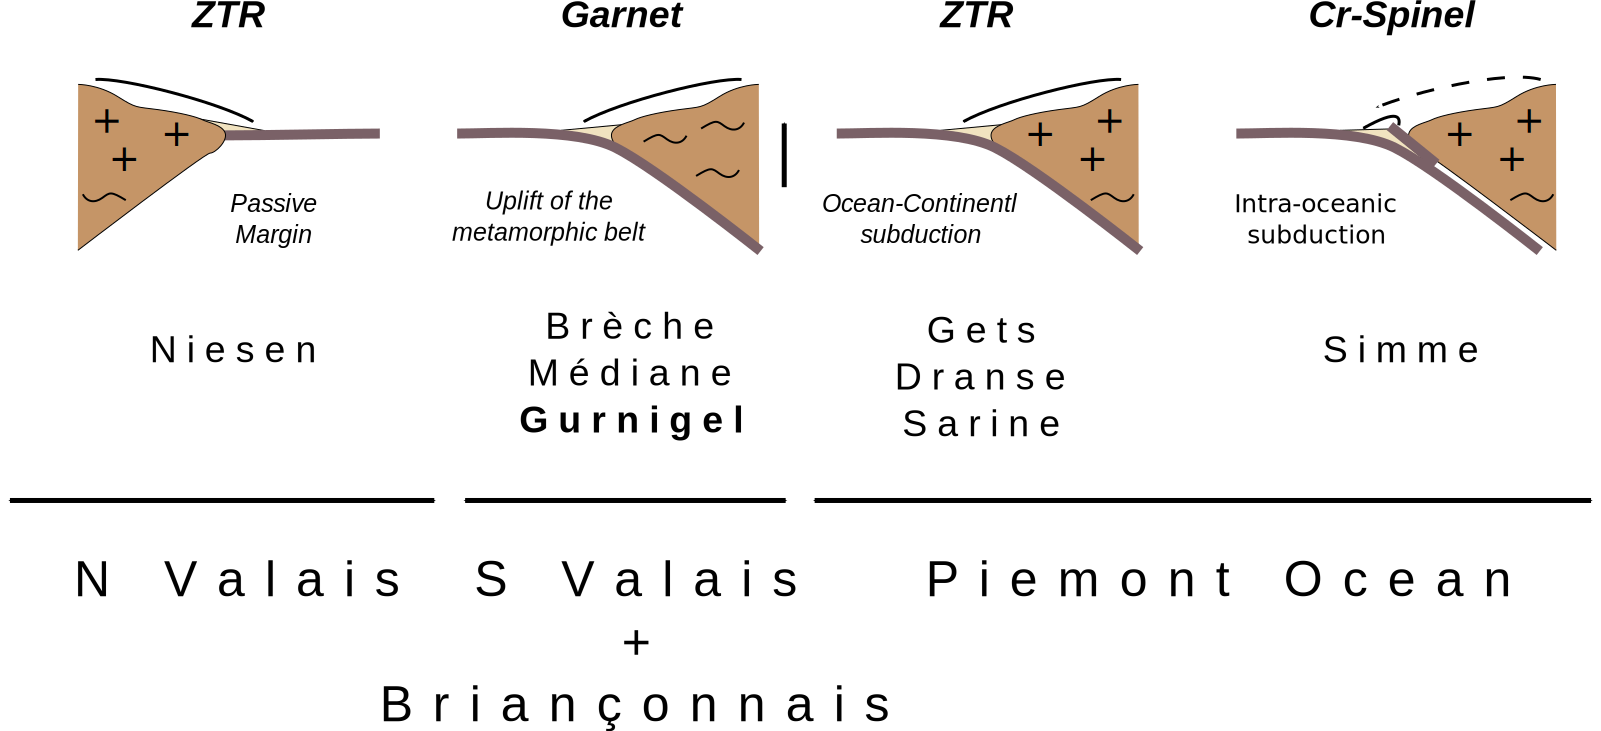
\includegraphics[width=\textwidth]{Fig21.pdf}
		\caption{Synthetic model of the evolution of tectonic settings during the Tethyan close-up and the respective heavy-mineral provinces of \citep{Wildi1985}}
		\label{fig:Fig21}
	\end{figure}
	}

\subsection{Geotectonic model of the Voirons Flysch}

The petrographic and mineralogical data presented in this study show that, like the other flyschs of the Gurnigel nappe, the constituent material of the Voirons Flysch originates from the southern margin of the Alpine Tethys \citep{Butler2011}. Five major age populations were identified in the detrital zircons (610-550, 510-490, 468-425, 346-315, 205 Ma; Fig. 23; \citealp{Butler2011}) corresponding to the different palaeogeographic province of the Tethyan realm. The palaeocurrent pattern of the Gurnigel nappe indicates a northern direction which is deflected eastward along the oceanic trench \citep{Caron1980,Winkler1984,Wildi1985} (Fig. 24). Both the palaeocurrent pattern and biostratigraphy further suggest a westward migration of the detrital source linked to the scissor closure of the basin \citep{Winkler1984}. Moreover, biostratigraphic work by \citep{Ujetz1996} and, more recently, \citep{Ospina-Ostios2013} showed that the sedimentation of this flysch took place in a time interval between the Middle Eocene and the Late Eocene/Early Oligocene. In this period, the sedimentary accretionary prism comprised the Briançonnais and Piemont sedimentary covers (Mosar et al, 1996, Fig. 7) and, in the highest position, of the Sesia-Dent Blanche nappe \citep{Schmid1996,Handy2010} (Fig. 25). The latter of which was partially obducted and formed the back stop of the Alpine Tethys accretionary prism \citep{Stampfli1998,Manzotti2014}. This prism was separated from the Southern Alps by the Periadriatic fault. Hence, no sediments from the Southern Alps could contribute to flysch deposition in the Alpine Tethys, except for those already reworked during the initiation of subduction (e.g. the Simme Flysch) explaining how Southern Alps-derived volcanic grains of Triassic age (205 Ma peak, Fig. 23) occur in the Gurnigel nappe \citep{Butler2011} and Médianes Flysch \citep{Beltran-Trivino2013}. In addition, the detrital zircon population pertaining to 468-425 Ma peak can also be related to the Southern Alps.\par
\medskip
The Sesia-Dent Blanche nappe is composed of an igneous basement and of sedimentary covers metamorphosed during the Late Cretaceous \citep{Manzotti2014}. It formed the metamorphic belt of the Tethyan accretionary prism (Figs. 23 and 24). The geochemistry of garnets from the Voirons Flysch suggests derivation from metasedimentary rocks and (metamorphosed?) igneous rocks of similar composition to those described from the Sesia Dent-Blanche nappe (Fig. 22). Alm-Prp-Grs and Grs-And grains are indeed reported in metapelite; metabasite and calcsilicate rocks respectively from this unit \citep{DalPiaz1983}. The former may also derive from recycled kinzigite preserved in the Eclogitic Micaschists Complex. A potential clinopyroxene-rich amphibolite from the Valpelline serie is also envisaged considering the metabasite source. Our data is in agreement with the garnet geochemical data of \cite{Kirst2014} from metasedimentary rocks of the Becca d’Aver continental sliver. Almandine-rich garnet is also reported in the Lombardian Flysch of the Southern Alps \citep{Bernoulli1990} corroborating that the Sesia Dent-Blanche nappe could be the source of garnets. Despite tourmaline being widespread in the Alps, geochemical data are scarce, preventing constraints on their origin. Finally, the few geochronological data (Manzotti et al., 2014 and Fig. 23) obtained from the Sesia-Dent Blanche nappe could correspond to the 468–425 Ma range reported by \cite{Butler2011}.\par
Rare andesite lithoclasts observed in the Voirons Sandstone Fm. (\citealp{Ospina-Ostios2013}, Fig. 4) cannot originate from the Sesia Dent-Blanche nappe due to the Oligocene age of the andesite layers from the external part of the Sesia-Lanzo unit \citep[and references therein]{Venturelli1984}. Nevertheless, Upper Carboniferous–Permian volcanic deposits relating to the Variscan orogeny \citep{Cortesogno1998a} are a potential source of andesite grains. Volcanic Upper Carboniferous–Permian units are reported from (1) the Ligurian Alps and Sardinia in the Briançonnais domain \citep{Cortesogno1998a,Decarlis2013} and the Siviez-Mischabel nappe \citep{Sartori2006}, and (2) the Southern Alps \citep{Cortesogno1998a} through the Simme nappe. Most of this event may have been poorly preserved in detrital zircon or poorly contribute to the detrital sedimentation. Hence, the 310-260 Ma interval constitutes secondary peak and rarely high frequency peak \citep[see sample 11EB07 in 280-300 Ma range for the latter]{Butler2011}. However, the oldest component may represent or at least contribute to the 346-315 Ma population of the detrital zircon \citep[Fig. 23]{Butler2011}. A derivation from a volcanic arc developed along the southern Tethyan margin during the subduction of the Piemont Ocean \citep{Gasinski1997} is excluded on the basis of a lack of coeval ages in detrital zircon \citep{Butler2011,Beltran-Trivino2013}, and bentonite layers \citep{Winkler1985a,Winkler1990} might derive from the British Paleogene Igneous Province \citep{Koch2015}.\par
Likewise, the black sandstones pebbles of Paleozoic age (Fig. 6b) reported from the Vouan Conglomerate Fm. likely indicate an input from the Briançonnais basement. Such pebbles possibly originate from the Palaeozoic rift basin of the Zone Houillère \citep{Fabre1961}. In addition, recent detrital zircon geochronological data from the Dora Maira massif and the Zone Houillère \citep{Manzotti2016} constrain the magmatic events between 330-340 Ma which correspond to the 346-315 Ma peak (Fig. 23). Moreover, a similar almandine-rich garnet geochemistry is reported from the Briançonnais basement (Fig. 22). An Alm-Prp-Grs composition is reported from the Siviez-Mischabel nappe \citep{Thelin1990} as well as Alm-Sps composition from the Zone Houillère \citep{Bucher2007} and Pontis nappe \citep{Giorgis1999}. However, pyrope grains documented in the Dora Maira massif by \citep{Schertl1991} are absent. The combination of data suggests that the Briançonnais basement during its subduction is a likely detrital source (Fig. 24). Nevertheless, distinguishing this detrital source from the Sesia Dent-Blanche nappe remains problematic and might be resolved using additional analysis such as garnet geochronology \citep{Baxter2013}.\par
\medskip

\afterpage{
	\begin{figure}[htp!]
		\centering
		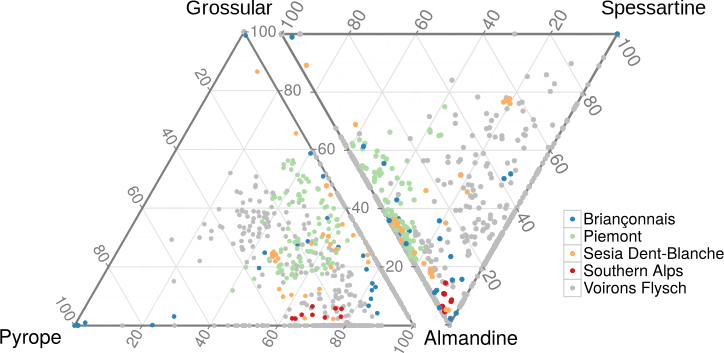
\includegraphics[width=\textwidth]{Fig22.pdf}
		\caption{Major garnet end-member ternary diagram of middle to upper Penninic domains based on compilation of \citep{Stutenbecker2016}. Briançonnais: \citep{Thelin1990}, \citep{Schertl1991}, \citep{Giorgis1999}, \citep{Bucher2007}; Piemont: \citep{Oberhansli1980}, \citep{Cartwrigth2002}, \citep{Bucher2009}, \citep{Weber2015}; Sesia–Dent Blanche: \citep{DalPiaz1983}, \citep{Gardien1994}, \citep{Kirst2014}; Southern Alps: \citep{Hunziker1980}} 
		\label{fig:Fig22}
	\end{figure}
	}
\afterpage{
	\begin{figure}[htp!]
		\centering
		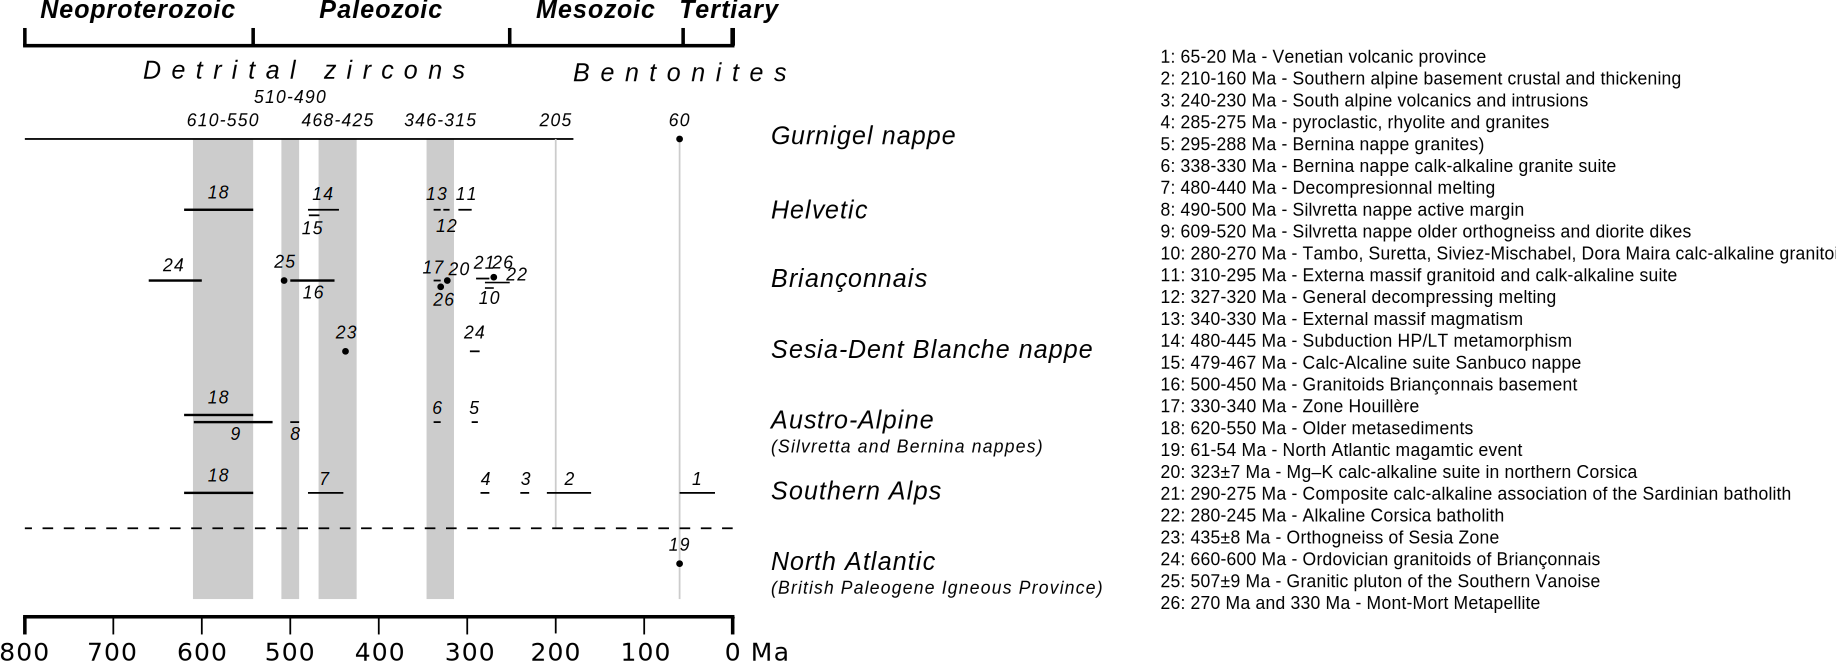
\includegraphics[width=\textwidth]{Fig23.pdf}
		\caption{Major U/Pb age peaks of the detrital zircons \citep{Butler2011} and bentonites \citep{Koch2015}. Data are compared to the major magmatic events in the Tethyan realm based on the modified compilation of \citep{Butler2011}. \cite{Butler2011}: 1–16; \citep{Schaltegger1999}: 18–24,25; \citep{Koch2015}: 19; \citep{Cortesogno1998a}: 20–22; \citep{Manzotti2014}: 23; \citep{Bussy1996}: 26} 
		\label{fig:Fig23}
	\end{figure}
	}

Finally, the older detrital zircon geochronological data are widespread distributed and hence cannot constrain the detrital source. The 510-490 Ma range (Fig. 23) is reported from the Briançonnais domain and the Austro-alpine Silvretta nappe \citep{Schaltegger1999}. The 610-550 Ma range (Fig. 23) is linked to the oldest meta-sediments in the Briançonnais, Austro-alpine and Southern Alps \citep{Schaltegger1999}. In addition, although they match with several peaks (610-550, 468-425 and 346-315 Ma, Fig. 23), zircon ages from the northern Tethyan margin are irrelevant since no southward palaeocurrent is described in the Gurnigel nappe.\par
\medskip
The exhumed metamorphic lithologies of the Sesia-Dent Blanche nappe, and to a lesser extent of the Briançonnais basement, could likely represent the Basement uplift tectonic setting (Dickinson et al., 1985) or the Axial belt provenance \citep{Garzanti2004,Garzanti2007b,Garzanti2010} of the Feldspathic petrofacies (Fig. 9). This is in agreement with the feldspar dominated and garnet-rich detrital composition of modern fluvial sediments shed by the Dent Blanche nappe \citep{Garzanti2010}. The accretionary prism fed the flysch deposits with reworked detrital grains of various lithologies (calcareous to crystalline rocks) (Fig. 24). These reworked sediments were depleted in unstable grains which gave them a mature composition \citep{Velbel1985}. The resulting detrital composition reflects the Clastic wedge provenance of the Garzanti model \citep{Garzanti2007b} and the Transitional continental to Mixed tectonic setting \citep{Dickinson1985} of the Quartzose petrofacies (Fig. 9).\par
\medskip

\afterpage{
	\begin{figure}[htp!]
		\centering
		\includegraphics[width=0.5\textwidth]{Fig24.pdf}
		\caption{Palaeogeographic model of the Voirons Flysch and its two different detrital sources} 
		\label{fig:Fig24}
	\end{figure}
	}
\afterpage{
	\begin{figure}[htp!]
		\centering
		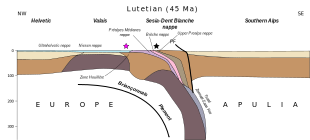
\includegraphics[width=\textwidth]{Fig25.pdf}
		\caption{Cross section of the Tethyan realm during the Lutetian \citep[modified]{Handy2010}. The stars indicates the paleogeographic location of the Voirons Flysch considering a Paleocene to Middle Eocene (\emph{black}) and Middle to Late Eocene age (\emph{purple})} 
		\label{fig:Fig25}
	\end{figure}
	}

This palaeogeographic model of the Voirons Flysch (Fig. 24) differs from the well-accepted model applied to the other flyschs from the Gurnigel nappe \citep{Winkler1983,Winkler1984,Caron1989}. The latter considers a Maastrichtian to Lutetian age \citep{Stuijvenberg1979,Stuijvenberg1980b,Winkler1983,Winkler1984}, and constrains the deposition of the Gurnigel flyschs in a Piemont Ocean characterised by a sedimentary accretionary prism that was smaller at that time than in the Middle Eocene to Late Eocene/Early Oligocene (Fig. 25). Based on the palaeogeographic reconstructions for the Early Cenozoic \citep{Schmid1996,Handy2010}, the suggested detrital sources for these flyschs are restricted to the Sesia Dent-Blanche nappe and the Upper Prealps nappes (Fig. 25). The dispute thus lies on the younger age obtained for the Voirons Flysch \citep{Ujetz1996,Ospina-Ostios2013}, which precludes deposition in the Piemont domain. Further biostratigraphic investigations are needed to clarify the palaeogeographic locations for the entire Gurnigel nappe. As long as the biostratigraphy of this nappe is not completely resolved, the relationship of the Voirons Flysch with the rest of the Gurnigel nappe, and their respective palaeogeographic locations, remain a matter of debate.

\subsection{Temporal evolution of the detrital inputs}

The correlation of the petrofacies of the Voirons Flysch with the stratigraphy shows a temporal variation in the sediment supplies (Fig. 17a) as already suggested by \citep{Winkler1984} for the rest of the Gurnigel nappe. Deposition began during the Middle Eocene with the Quartzose petrofacies in the Voirons Sandstone Fm. The source of the Feldspathic petrofacies was barely active at that time. In Late Eocene, inputs from the Feldspathic petrofacies markedly increased and alternated with those from the Quartzose petrofacies which progressively decreased. The fading of the Quartzose petrofacies concurred with the progradation of the turbiditic system and the deposition of the Vouan Conglomerate Fm. During these events, the source of the Quartzose petrofacies was either inactive or the detritus was shed to a different basin which remains unknown. The sharp contact between the Vouan Conglomerate Fm. and the Boëge Marl Fm. marks an abrupt modification both in the turbiditic system (development of a starved system) and in the sediment supply (the Quartzose petrofacies returns as the dominant supply) which may be related to major tectonic events. Finally, the gradual evolution towards the Bruant Sandstone Fm. indicates a steady-state system with an increase of sand-shale ratio dominated by the Quartzose petrofacies and sporadic inputs of the Feldspathic petrofacies.

\section{Conclusions}

Our study of the Voirons Flysch complements the existing dataset on the petrography of the flyschs from the Gurnigel nappe, and offers a new interpretation of the provenance of its constituent material.

	\begin{enumerate}
		\item In contrast to the other flysch units from the Gurnigel nappe, two distinctive sources have been identified in the Voirons Flysch,
		\begin{itemize}
			\item The Quartzose petrofacies is the major detrital source. It is similar to the provenances described elsewhere in the Gurnigel nappe. It is a quartz-rich assemblage with sedimentary to magmatic lithoclasts and a heavy-mineral assemblage dominated by ZTR + apatite. The most salient clasts in the conglomerate layers are pink granite fragments. The lithic composition variation reflects polycyclic sedimentary inputs corresponding to a Transitional continental block tectonic setting \citep{Dickinson1979a} or a Clastic wedge provenance \citep{Garzanti2007b}.
			\item The Feldspathic petrofacies represents a subordinate source in the Voirons Flysch, and has up to now not been identified elsewhere in the Gurnigel nappe. The Feldspathic petrofacies is mostly restricted to the Vouan Conglomerate Fm. Rock-fragment composition is characterised by black sandstones of Paleozoic age in conglomeratic layers. Garnet dominates the heavy-mineral assemblage, and metamorphic lithoclasts describe an Axial belt provenance \citep{Garzanti2007b} or a Basement uplift tectonic setting \citep{Dickinson1979a} considering the feldspar-rich composition. Samples distribution shows punctual inputs of this secondary detrital source during deposition of the Quartzose petrofacies.
		\end{itemize}
		\item The random deposition of the Feldspathic petrofacies within lithologic units dominated by the Quartzose petrofacies, as well as the interfingering contact between the Voirons Sandstone Fm. and the Vouan Conglomerate Fm. confirm the stratigraphic nature of the contacts within the Voirons Flysch.
		\item A comparison of the Voirons Flysch with the Sarine and Dranses flyschs shows a similar quartz-rich composition, which indicates a similar source along the southern Tethyan margin and/or reworking of the latter deposits in the former.
		\item A palaeogeographic location of the Voirons Flysch in the Valais domain is suggested considering (1) the Middle Eocene to Late Eocene/Early Oligocene age obtained from planktonic foraminifera biostratigraphy \citep{Ujetz1996,Ospina-Ostios2013}, (2) the marked similarity of the black sandstone lithoclasts of Paleozoic age found in the Vouan Conglomerate Fm. with the Zone Houllière, (3) the resemblance of the Feldspathic petrofacies with the Médianes Flysch and (4) a potential Briançonnais source for the andesite rock-fragments.
		\item Our palaeogeographic model suggests that the Voirons Flysch was fed by the reworking of the sedimentary accretionary prism (Quartzose petrofacies) including the older Prealps nappes and by intermittent inputs from the Sesia Dent-Blanche nappe and possibly from the Briançonnais (Feldspathic petrofacies). However, identifying the detritus derived from the Briançonnais basement and that originating from the Sesia Dent-Blanche nappe is not straightforward. More accurate analysis (e.g. garnet geochronology) will be necessary to emphasise the detrital inputs from the Briançonnais units.
		\item Our presented palaeogeographic model for the Voirons Flysch might eventually be applied to the other flyschs of the Gurnigel nappe if future biostratigraphic studies, possibly based on planktonic foraminifers, extend the Middle Eocene to Late Eocene/Early Oligocene age obtained for the Voirons Flysch to all deposits forming the Gurnigel nappe. Thus, further biostratigraphic investigations are urgently needed to clarify this palaeogeographic conundrum.
	\end{enumerate}

\section*{Acknowledgements}

We thank François Gischig (University of Geneva) for technical help with thin sections and Dr. Mario Sartori (University of Geneva) for fruitful conversations. We are grateful to Franz Neubauer and an anonymous reviewer for constructive comments on an earlier manuscript.

\bibliographystyle{apalike}
\bibliography{Ragusa2017a}

\end{document}
